%!TEX TS-program = xelatex
% !TeX program = xelatex
%!TEX encoding = UTF-8 Unicode
%----------------------------------------------------------------------------------------
%   Доорх хэсгийг өөрчлөх шаардлагагүй
%----------------------------------------------------------------------------------------
\documentclass[12pt,A4]{report}

\usepackage{fontspec,xltxtra,xunicode}
\setmainfont[Ligatures=TeX]{Times New Roman}
\setsansfont{Arial}

% \usepackage[utf8x]{inputenc}
% \usepackage[mongolian]{babel}
%\usepackage{natbib}
\usepackage{geometry}
%\usepackage{fancyheadings} fancyheadings is obsolete: replaced by fancyhdr. JL
\usepackage{fancyhdr}
\usepackage{float}
\usepackage{afterpage}
\usepackage{graphicx}
\usepackage{amsmath,amssymb,amsbsy}
\usepackage{dcolumn,array}
\usepackage{tocloft}
\usepackage{dics}
\usepackage{nomencl}
\usepackage{upgreek}
\newcommand{\argmin}{\arg\!\min}
\usepackage{mathtools}
\usepackage[hidelinks]{hyperref}

\usepackage{algorithm}
\usepackage{algpseudocode}

\usepackage{listings}
\DeclarePairedDelimiter\abs{\lvert}{\rvert}%
\makeatletter
\usepackage{caption}
\captionsetup[table]{belowskip=0.5pt}
\usepackage{subfiles}

\usepackage{listings}

\usepackage{color}
\definecolor{lightgray}{rgb}{.9,.9,.9}
\definecolor{darkgray}{rgb}{.4,.4,.4}
\definecolor{purple}{rgb}{0.65, 0.12, 0.82}

\lstdefinelanguage{TypeScript}{
  keywords={abstract, any, as, boolean, break, case, catch, class, console, 
    const, continue, debugger, declare, default, delete, do, else, enum, export, 
    extends, false, finally, for, from, function, get, if, implements, import, in, 
    infer, instanceof, interface, keyof, let, module, namespace, never, new, null, 
    number, object, package, private, protected, public, readonly, require, return, 
    set, static, string, super, switch, symbol, this, throw, true, try, type, typeof, 
    undefined, unique, unknown, var, void, while, with, yield, async, await},
  keywordstyle=\color{blue}\bfseries,
  ndkeywords={class, export, boolean, throw, implements, import, this},
  ndkeywordstyle=\color{darkgray}\bfseries,
  identifierstyle=\color{black},
  sensitive=false,
  comment=[l]{//},
  morecomment=[s]{/*}{*/},
  commentstyle=\color{purple}\ttfamily,
  stringstyle=\color{red}\ttfamily,
  morestring=[b]',
  morestring=[b]"
}

\lstset{
   language=TypeScript,
   backgroundcolor=\color{lightgray},
   extendedchars=true,
   basicstyle=\footnotesize\ttfamily,
   showstringspaces=false,
   showspaces=false,
   numbers=left,
   numberstyle=\footnotesize,
   numbersep=9pt,
   tabsize=2,
   breaklines=true,
   showtabs=false,
   captionpos=b
}
\lstdefinelanguage{yaml}{
  keywords={true,false,null,y,n},
  keywordstyle=\color{darkgray}\bfseries,
  basicstyle=\ttfamily\footnotesize,
  sensitive=false,
  comment=[l]{\#},
  morecomment=[s]{/*}{*/},
  commentstyle=\color{purple}\ttfamily,
  stringstyle=\color{blue}\ttfamily,
  morestring=[b]',
  morestring=[b]",
  breaklines=true,
  breakatwhitespace=true
}
\renewcommand{\lstlistingname}{Код}
\renewcommand{\lstlistlistingname}{\lstlistingname ын жагсаалт}

\usepackage{color}
\definecolor{codegreen}{rgb}{0,0.6,0}
\definecolor{codegray}{rgb}{0.5,0.5,0.5}
\definecolor{codepurple}{rgb}{0.58,0,0.82}
\definecolor{backcolour}{rgb}{0.99,0.99,0.99}
 
\lstdefinestyle{mystyle}{
    basicstyle=\ttfamily\small,
    backgroundcolor=\color{backcolour},   
    commentstyle=\color{codegreen},
    keywordstyle=\color{magenta},
    numberstyle=\tiny\color{codegray},
    stringstyle=\color{codepurple},
    %basicstyle=\footnotesize,
    breakatwhitespace=false,         
    breaklines=true,                 
    captionpos=b,                    
    keepspaces=false,                 
    numbers=left,                    
    numbersep=10pt,                  
    showspaces=false,                
    showstringspaces=true,
    showtabs=false,                  
    tabsize=2
}
 
\lstset{style=mystyle, label=DescriptiveLabel} 

\let\oldabs\abs
\def\abs{\@ifstar{\oldabs}{\oldabs*}}
\makenomenclature
\begin{document}


%----------------------------------------------------------------------------------------
%   Өөрийн мэдээллээ оруулах хэсэг
%----------------------------------------------------------------------------------------

% Дипломийн ажлын сэдэв
\title{Криптографын зарим алгоритм, программ}
% Дипломын ажлын англи нэр
\titleEng{Some algorithms and programs for cryptography}
% Өөрийн овог нэрийг бүтнээр нь бичнэ
\author{Даянгийн Балжинням}
% Өөрийн овгийн эхний үсэг нэрээ бичнэ
\authorShort{Д. Балжинням}
% Удирдагчийн зэрэг цол овгийн эхний үсэг нэр
\supervisor{Д. Гармаа}
% Хамтарсан удирдагчийн зэрэг цол овгийн эхний үсэг нэр
\cosupervisor{Н. Оюун-Эрдэнэ}

% СиСи дугаар 
\sisiId{20B1NUM0563}
% Их сургуулийн нэр
\university{МОНГОЛ УЛСЫН ИХ СУРГУУЛЬ}
% Бүрэлдэхүүн сургуулийн нэр
\faculty{ХЭРЭГЛЭЭНИЙ ШИНЖЛЭХ УХААН, ИНЖЕНЕРЧЛЭЛИЙН СУРГУУЛЬ}
% Тэнхимийн нэр
\department{МЭДЭЭЛЭЛ, КОМПЬЮТЕРИЙН УХААНЫ ТЭНХИМ}
% Зэргийн нэр
\degreeName{Баклаврын судалгааны ажил}
% Суралцаж буй хөтөлбөрийн нэр
\programeName{Програм хангамж(D061302)}
% Хэвлэгдсэн газар
\cityName{Улаанбаатар}
% Хэвлэгдсэн огноо
\gradyear{2023 оны 11 сар}


%----------------------------------------------------------------------------------------
%   Доорх хэсгийг өөрчлөх шаардлагагүй
%----------------------------------------------------------------------------------------
%----------------------Нүүр хуудастай хамаатай зүйлс----------------------------
\pagenumbering{roman}
\makefrontpage
\maketitle

\doublespace

% Decleration
\begin{huge}
	\textbf{Зохиогчийн баталгаа}
\end{huge} \\ \ \\
\doublespace
Миний бие \@author \ "\@title" \ сэдэвтэй судалгааны ажлыг гүйцэтгэсэн болохыг зарлаж дараах зүйлсийг баталж байна:
\begin{itemize}
	\item Ажил нь бүхэлдээ эсвэл ихэнхдээ Монгол Улсын Их Сургуулийн зэрэг горилохоор дэвшүүлсэн болно.
	\item Энэ ажлын аль нэг хэсгийг эсвэл бүхлээр нь ямар нэг их, дээд сургуулийн зэрэг горилохоор оруулж байгаагүй.
	\item Бусдын хийсэн ажлаас хуулбарлаагүй, ашигласан бол ишлэл, зүүлт хийсэн.
	\item Ажлыг би өөрөө (хамтарч) хийсэн ба миний хийсэн ажил, үзүүлсэн дэмжлэгийг дипломын ажилд тодорхой тусгасан.
	\item Ажилд тусалсан бүх эх сурвалжид талархаж байна.
\end{itemize}
\

Гарын үсэг: \underline{\hspace{5cm}}

Огноо: 	\ \ \underline{\hspace{3cm}}

% Гарчгийг автоматаар оруулна
\setcounter{tocdepth}{1}
\tableofcontents

% Зургийн жагсаалтыг автоматаар оруулна
\listoffigures

% Хүснэгтийн жагсаалтыг автоматаар оруулна
\listoftables

% Кодын жагсаалтыг автоматаар оруулна
\lstlistoflistings

% This puts the word "Page" right justified above everything else.
\newpage
%% \addtocontents{lof}{Зураг~\hfill Хуудас \par}
\newpage
%% \addtocontents{lot}{Хүснэгт~\hfill Хуудас \par}

\renewcommand{\cftlabel}{Зураг}


\doublespace
\pagenumbering{arabic}


% Удиртгалыг оруулж ирэх ба abstract.tex файлд удиртгалаа бичнэ
\begin{abstract}
	\setcounter{secnumdepth}{0}
	Энэхүү дипломын ажилд криптографын янз бүрийн алгоритм, программуудыг системтэйгээр судалсан бөгөөд үндсэн зорилго нь тэдгээрийн үндсэн бүтэц, үйл ажиллагааны механизм, практик хэрэглээг ойлгох явдал байв. Энэхүү судалгааны ажилд уламжлалт болон шинээр гарч ирж буй криптографын алгоритмуудыг судалж, гүйцэтгэл, аюулгүй байдал, үр ашигтай байдалд үндэслэн харьцуулсан судалгааг хийв.\\

	Энэхүү судалгаанд өгөгдлийн шифрлэлтийн стандарт (DES), дэвшилтэт шифрлэлтийн стандарт (AES), Ривест-Шамир-Адлеман (РСА (RSA)), эллиптик муруй криптографи (ECC) зэрэг тэгш хэмтэй болон тэгш хэмт бус криптографын алгоритмуудыг нарийвчлан судалсан.\\

	Төгсөлтийн ажлын практик хэсэгт хэд хэдэн криптографын программуудыг боловсруулж харьцуулсан ба орчин үеийн стандартыг хангасан тоон гарын үсгийн системийг үүлэн технологит суурилан бүтээсэн.
	\section{Зорилго}
	Энэхүү ажилд үүлэн технологит суурилсан тоон гарын үсгийн системийг бүтээж хэрэглэгчэд өөрсдийн цахим гарын үсгээр баталгаажсан файлуудыг интернэтэд хуваалцах боломжийг бүрдүүлэх гол зорилго зорилго тавьсан болно.
	\section{Зорилт}
	\begin{enumerate}
		\item Криптографын сонгодог алгоритмуудыг судлах, эзэмших
		\item Криптографын сонгодог алгоритмууд болон үүлэн технологид суурилсан тоон гарын үсгийн систем бүтээх
		\item Бүрэн бүтэн, хөндөгдөөгүй, эх сурвалжтай файлыг хуваалцах боломжийг бүрдүүлэх
	\end{enumerate}
	\section{Үндэслэл}
	Цахим харилцаа холбоо хурдацтай хөгжиж буй өнөөгийн нийгэмд, хуулийн дагуу хүчин төгөлдөр бичиг баримтыг интернэт сүлжээг ашиглан хуваалцах хэрэг байна. Гэсэн хэдий ч Монголд үүлэн дээр суурилсан тоон гарын үсгийн систем байхгүйгээс хэрэглэгчэд нийцгүй байгаа нь харагдаж байна.

	Дэлхийн банкны мэдээллээр Монгол Улсын иргэдийн дийлэнх хувь нь (2021 оны байдлаар 81.61\%) интернэт хэрэглэгч байгаа нь ийм системийн боломжит цар хүрээг харуулж байна. \footnote{Дэлхийн банкны судалгаа: \url{https://data.worldbank.org/indicator/IT.NET.USER.ZS?end=2021&locations=MN}}
	
	Түүнчлэн, одоо байгаа Клиент программууд нь Windows үйлдлийн системд зориулагдсан байдаг. Энэхүү Windows төвтэй арга нь нийцтэй байдлын асуудалд хүргэдэг. StatCounter Global Stats-аас гаргасан мэдээллээс харахад 2023 оны байдлаар дэлхий даяар үйлдлийн системийн зах зээлийн 30 орчим хувийг macOS болон Linux зэрэг Windows бус платформууд эзэлж байна.\footnote{Үйлдлийн системийн судалгаа: \url{https://gs.statcounter.com/os-market-share/desktop/worldwide}}
	
	Эдгээрийг авч үзвэл хэрэглэгчдийн олон талт хэрэгцээнд нийцсэн үүлэн технологит суурилсан тоон гарын үсгийн системийг хөгжүүлэх шаардлагатай байгаа нь харагдаж байна.

	%	\setcounter{secnumdepth}{0} reverse this command
	\setcounter{secnumdepth}{2}

\end{abstract}



%----------------------------------------------------------------------------------------
%   Дипломын үндсэн хэсэг эндээс эхэлнэ
%----------------------------------------------------------------------------------------
%\addcontentsline{toc}{part}{БҮЛГҮҮД}
% Шинэ бүлэг
\chapter{Онолын судалгаа}
\section{Тэгш хэмт крифтограф}
Тэгш хэмт крифтографт шифрлэлт болон шифр тайлах түлхүүрүүд адил байна. Тэгш хэмт алгоритм нь Тэгш бус хэмт шифрлэлтээс харьцангуй хурдан ажилдаг. Гэвч нууцалсан мэдээллийг тайлж унших түлхүүр болон нууцлах түлхүүр адилхан байх нь харилцагч талууд урьдчилан түлхүүрээ хоорондоо тохиролцох шаардлагыг гаргаж ирдэг. Энэ нь сул тал болох эрсдэлтэй. Хэрвээ гуравдагч этгээд түлхүүрийг олж авбал бүх нууцалсан мэдээллийг үзэх боломжтой болох юм.

Хамгийн түгээмэл хэрэглэгддэг тэгш хэмт шифрлэлтийн алгоритм бол Бельгийн криптографич Жоан Даемен, Винсент Рижмен нарын боловсруулсан Advanced Encryption Standard (AES) юм. AES нь хуучин Data Encryption Standard (DES)-ийг сольсон бөгөөд одоо дэлхий даяар ашиглагдаж байна.\cite{AES}
\subsection{Блокон шифрлэлт}

Хэрвээ эх ба шифрлэгдсэн тексүүдийн огторгуй нь ямар нэг $\sum_{}^{n}$ олонлог байвал тухайн криптографыг блокон шифрлэлт гэнэ. Блокон шифрлэлтэд өгсөн мэдээг тэнцүү \textit{n} урттай хэсгүүдэд хуваан шифрлэдэг.\cite{intro_crypo}

Блок шифрт энгийн текстийн блокийг бүхэлд нь авч, шифрлэгдсэн текстийн блокийг үүсгэхэд ашигладаг. Блокийн хэмжээг ерөнхийдөө шифрийн алгоритмаар тодорхойлно. Ихэнх блок шифрүүдийн хувьд энэ нь ихэвчлэн 64 эсвэл 128 бит байдаг ба зарим тохиолдолд нууцлалыг нэмэх зорилгоор 256, 512 бит ч байж болдог.


Хоёр төрлийн алгоритм ашиглах ба нэг нь шифр хийхэд нөгөө нь тайлахад ашиглагддаг. Эдгээр нь \textit{n} урттай бит болон \textit{k} бит урттай түлхүүрийг авч \textit{n} бит урттай блок үүсгэнэ.\\$E: \{0,1\}^k \times \{0,1\}^n \rightarrow \{0,1\}^n$.
	Тайлах алгоритм \textit{D}-г нууцлах функцийн урвуу гэж тодорхойлж болно.\\ $D: \{0,1\}^k \times \{0,1\}^n \rightarrow \{0,1\}^n$\\
$\forall k \in \{0,1\}^k, \forall m \in \{0,1\}^n, D(k, E(k, m)) = m$\\
	\cite{modern_crypto}

	\subsection{Урсгалын шифрлэлт}
	Урсгалын шифрлэлт гэдэг нь өгөгдлийг урсгал маягаар нэг дор нэг битийг Криптографын алгоритм болон түлхүүрээ ашиглан шифрлэх арга юм. Урсгалын шифрийн давуу тал нь блок шифрлэлтээс харьцангуй хурдан ажиллахаас гадна, хэрэгжүүлэлтэд бага код ордог билээ. Гэсэн хэдий ч орчин үед түгээмэл ашиглагдахаа больсон ба элдэв халдагад түгээмэл өртдөг нь үүнтэй холбоотой. Жишээ нь RC4 гэх Урсгалын шифрлэлтийн алгоритм нь WEB болон WPA хамгаалалтад ашиглагддаг байсан хэдий ч хангалттай сайн хамгаалалт болж чадахгүй байгаа тул, хэрэглээнээс халагдаж байна.

	\section{Өгөгдөл шифрлэлтийн стандарт}
	\subsection{DES алгоритм}
	DES (Data Encryption Standard) нь 1970-аад онд хөгжүүлэгдсэн тэгш хэмт блок шифрлэлтийн алгоритм юм. DES нь 64 бит урттай блок дээр ажиллах ба үүнийг 32-бит урттай хоёр хэсэг $L_{0}, R_{0}$ болгон хувааж, баруун талын 32-бит урттай хэсгийг олон янзын аргаар хувиргаж эцэст нь $L_{0}$-тэй XOR үйлдэл хийнэ. Арван зургаан үе хувиргалтын дараагаар $L_{0}, R_{0}$ нийлүүлж 64 бит шифрлэгдсэн блокийг үүсгэнэ.
	\subsubsection{Шинжүүд}
	\begin{enumerate}
		\item Түлхүүрийн урт: DES нь 56 битийн түлхүүрийг ашигладаг бөгөөд анхандаа хангалттай аюулгүй байдлыг хангадаг гэж бодож байсан ч одоо Brute Force халдлагад маш эмзэгт тооцогддог.
		\item Symmetric Encryption: DES нь шифрлэлт болон шифрийг тайлахад ижил түлхүүр ашигладаг. Тиймээс түлхүүрийг илгээгч, хүлээн авагч хоёулаа мэдэж, нууцлах ёстой.

		\item Блок шифр: DES нь тусдаа бит биш харин өгөгдлийн блокууд дээр ажилладаг. Энэ нь их хэмжээний өгөгдлийг шифрлэх шаардлагатай программуудад тохиромжтой.

		\item DES үйлдлүүд: DES нь  Electronic Codebook (ECB), Cipher Block Chaining (CBC), Cipher Feedback (CFB), Output Feedback (OFB), and Counter (CTR) зэрэг хэд хэдэн үйлдлийн горимыг дэмждэг.

		\item DES нь детерминистик: ижил текст болон ижил түлхүүрийн хувьд шифрлэгдсэн текст үргэлж ижил байх болно.
	\end{enumerate}
	хэдийгээр 3-DES гэж байдаг хэдий ч энэ нь тооцоолол ихээр шаарддаг тул цаашид ашиглагдах нь зогссон.

	\subsection{AES}
	АНУ-ын Стандарт, Технологийн үндэсний хүрээлэн (VIST) 1997 онд өгөгдөл нууцлалын стандарт (DES)-ыг сайжруулах ажлыг эхлүүлж 2001 онд В.Рижмень, Д.Дэймен нарын блокон шифрлэлтийн схемийг дэвшилтэт нууцлалын стандартаар зарласан.\cite{intro_crypo}

	AES нь орлуулах сэлгэлт (substitution-permutation) гэж нэрлэгддэг зарчим дээр суурилдаг бөгөөд программ хангамж болон техник хангамжийн аль алин дээр нь хурдан ажилдаг. Орчин үед шифрлэлтийг хурдан хийх зорилгоор техник хангамж дээр зөвхөн энэ алгоритмд зориулсан хэсэг хүртэл байдаг билээ.
	\subsubsection{Үндсэн үйлдэл}
	\begin{enumerate}
		\item \textbf{SubBytes:}
		      \begin{itemize}
			      \item Байт болгоны байрлалыг солино
			      \item Тухайн мөр баганын мэдээлэл солигдоно
		      \end{itemize}
		      \begin{figure}[h]
			      \centering
			      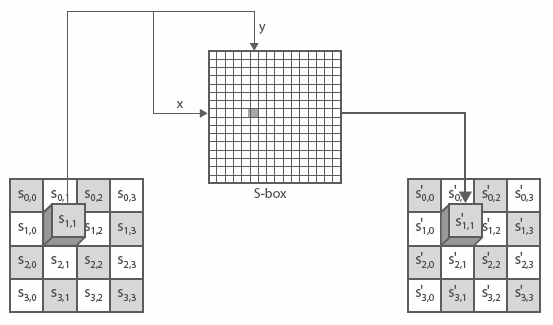
\includegraphics[scale=0.65]{assets/subbytes.png}
			      \caption{SubBytes үйлдэл}
			      \label{fig:subbytes}
		      \end{figure}
		\item \textbf{ShiftRows:}
		      \begin{itemize}
			      \item 1-р мөрийг шилжүүлэхгүй
			      \item 2–р мөрийн байтуудыг зүүн тийш 1 байт шилжүүлнэ
			      \item 3–р мөрийн байтуудыг зүүн тийш 2 байт шилжүүлнэ
			      \item 4–р мөрийн байтуудыг зүүн тийш 3 байт шилжүүлнэ
			      \item Тайлах үйлдлийг хийхдээ баруун тийш шилжүүлэх үйлдлийг хийнэ
		      \end{itemize}
		      \begin{figure}[h]
			      \centering
			      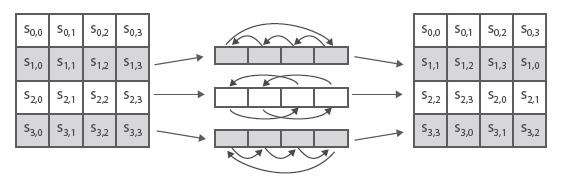
\includegraphics[scale=0.6]{assets/shiftrows.png}
			      \caption{ShiftRows үйлдэл}
			      \label{fig:shiftrows}
		      \end{figure}
		\item \textbf{MixColumns:}
		      \begin{itemize}
			      \item Багана бүр тус тусдаа холигдоно
			      \item Багана болгоны харгалзаа байтууд хоорондоо солигдоно
		      \end{itemize}
		      \begin{figure}[h]
			      \centering
			      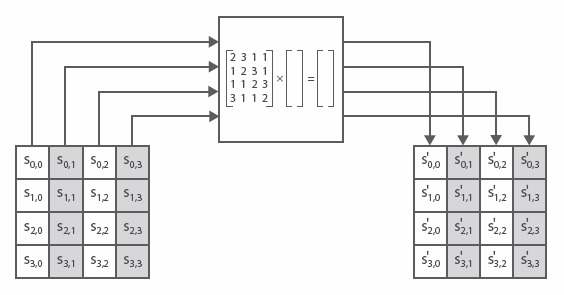
\includegraphics[scale=0.6]{assets/mixcolumns.png}
			      \caption{MixColumns үйлдэл}
			      \label{fig:mixcolumns}
		      \end{figure}
		\item \textbf{AddRoundKey:}
		      \begin{itemize}
			      \item 128 бит XOR үйлдлийг циклийн түлхүүрт ашиглана
			      \item Тайлах үйлдэл хийх бол эсрэгээр гүйцэтгэнэ
		      \end{itemize}
		      \begin{figure}[h]
			      \centering
			      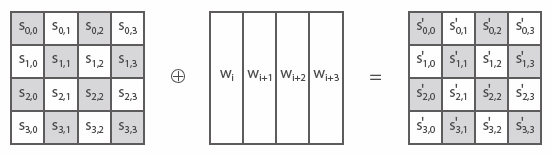
\includegraphics[scale=0.6]{assets/addroundkey.png}
			      \caption{AddRoundKey үйлдэл}
			      \label{fig:addroundkey}
		      \end{figure}
	\end{enumerate}

	\subsubsection{AES-ын нууцлалт}
	\begin{enumerate}
		\item шифрлэх блок ба түлхүүрийн урт, мөчлөгийн тоог сонгох. Шифрлэх блок ба түлхүүрийн урт нь 128, 192, 256 байт байж болох бөгөөд мөчлөгийн тоо нь харгалзан 10, 12, 14 байна.
		\item Шифрлэх текст, түлхүүрийн матриц \textit{T, W, K}-г үүсгэнэ.
		\item Эцсийн мөчлөгөөс бусад мөчлөгийн \textit{T, W, K} матрицуудад \textbf{AES}-н үндсэн үйлдлүүдийг дэс дараалан хийнэ. Харин эцсийн мөчлөгт Mix Columns үйлдлийг хийхгүй.
	\end{enumerate}
	% \subsubsection{Нууцын тайлалт}
	% 4x4 for matrix below
	\begin{center}
		$\begin{bmatrix}
				b_{0} & b_{4} & b_{8}  & b_{12} \\
				b_{1} & b_{5} & b_{9}  & b_{13} \\
				b_{2} & b_{6} & b_{10} & b_{14} \\
				b_{3} & b_{7} & b_{11} & b_{15} \\
			\end{bmatrix}$
	\end{center}
	\subsection{РСА (RSA)}
	РСА (RSA) нь анхны тооны өвөрмөц шинж чанарыг ашигладаг тэгш бус хэмтэй шифрлэлтийн арга юм. Анх 1977 онд танилцуулагдсан ба, өнөөг хүртэл хэрэглээнд хэвээр байгаа. Өнөөдрийн дэлхий даяар мөрдөгдөж байгаа стандарт нь хоёр анхны тооны үржвэр болох модулус нь 2048 бит хэмжээтэй байх ёстой. Энэ нь 617 оронтой тоо байна гэсэн үг юм.
	\begin{itemize}
		\item Хоёр анхны тоо болох $p$ болон $q$ сонгоно.
		\item $n = p*q$ утгыг олно.
		\item $\phi(n) = (p-1)*(q-1)$ утгыг олно.
		\item Дараах нөхцөлийг хангах $e$ тоог сонгоно $1 < e < \phi(n)$ ба хиех$(e, \phi(n)) = 1$.
		\item $d$ нь $d \equiv e^{-1} \mod \phi(n)$ гэж тодорхойлогдоно.
	\end{itemize}

	Нийтийн түлхүүр нь $(e, n)$ болох ба хувийн түлхүүр нь $(d, n)$ болно.\cite{РСА (RSA)}
	
\subsubsection{Нууцлал}
РСА (RSA) алгоритмын нууцлал маш том хэмжээний анхны тоог хоёр тооны үржигдэхүүн болгон задлах дээр тогтдог ба өнөөгийн бидний машины тооцон бодох чадал хараахан хангалттай биш байгаа юм.

\begin{table}[h!]
	\centering
	\caption{Муйхар хүчний алгоритм ашиглан РСА (RSA) нууцлалыг эвдэх нь \cite{Brute-force-РСА (RSA)}}
	\begin{tabular}{|c|c|c|c|}
	\hline
	n & p*q & Оролдого (Хайлт) & Хугацаа (секунд) \\
	\hline
	187 & $11 \times 17$ & 5 & $0.00344800949097$ \\
	913 & $11 \times 83$ & 5 & $0.00358390808105$ \\
	14041 & $19 \times 739$ & 8 & $0.004469871521$ \\
	557009 & $653 \times 853$ & 119 & $0.00167393684387$ \\
	9192907 & $937 \times 9811$ & 159 & $0.00201606750488$ \\
	37675201 & $3907 \times 9643$ & 540 & $0.0139532089233$ \\
	17614895377 & $40559 \times 434303$ & 4252 & $0.117401838303$ \\
	599855115407 & $694789 \times 863363$ & 56166 & $0.712327957153$ \\
	4684589242027 & $837533 \times 5593319$ & 66714 & $1.99000310898$ \\
	6833740248499 & $2565161 \times 2664059$ & 187492 & $2.51408982277$ \\
	91063247464523 & $9577907 \times 35324489$ & 188371 & $8.69724798203$ \\
	\hline
	\end{tabular}
	\end{table}

	Хамгийн сүүлд үржигдэхүүнд задалж чадсан буюу нууцлал нь амжилттай эвдэгдсэн нь РСА (RSA)-250 буюу 829 бит урттай байгаа юм. Фабрис Будот, Пьеррик Гаудри, Ауроре Гилевич, Надия Хенингер, Эммануэль Томе, Пол Циммерманн нараар ахлуулсан судлаачдын баг үүнийг 2020 онд гүйцэтгэсэн. Тооцоололд ойролцоогоор 2700 цөм жил \footnote{Цөм жил гэдэг нь CPU-ний нэг цөмийг бүтэн жил ашигласантай тэнцэнэ.} зарцуулагдсан бөгөөд шигших үе шат нь хуанлийн 35 долоо хоног янз бүрийн машинууд дээр хийгдсэн.

	\begin{figure}[h]
		\centering
		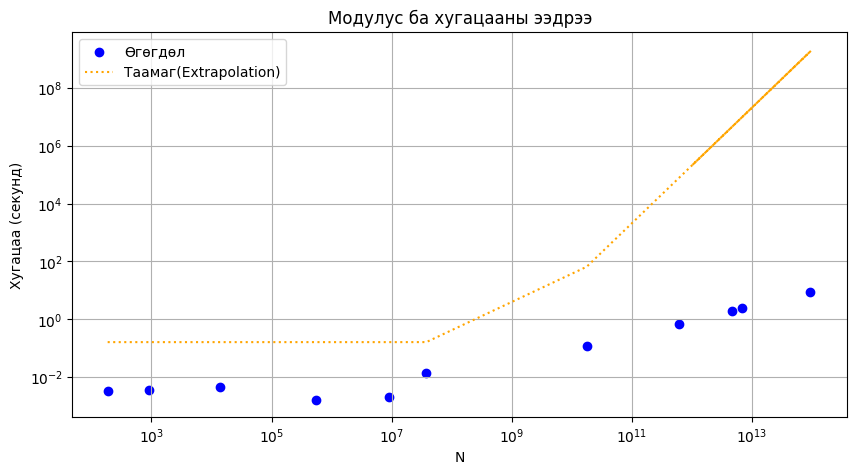
\includegraphics[scale=0.73]{assets/rsacomplexity.png}
		\caption{Хугацааны ээдрээ}
		\label{fig:rsacomplexity}
	\end{figure}

РСА (RSA) үржигдэхүүн задлах нь(factoring) цифрийн тоо нэмэгдэх тусам илтгэгч функцээр хугацааны ээдрээ тооцогдох тул одоогийн байдлаар РСА (RSA) 1024, РСА (RSA) 2048 нь хангалттай аюулгүй байгаа бөгөөд дэлхий нийтээрээ ашиглаж байна. Энэ нь дээрх диаграммаас харагдана.

\section[Тоон гарын үсэг]{Тоон гарын үсгийн стандартын судалгаа}
Хэдийгээр бүх цахим гарын үсэг нь DSS-ийн дүрмийг дагаж мөрдөх ёстой боловч тэдгээр нь бүгд адилхан биш юм. Баримт бичигт гарын үсэг зурахад ашиглаж болох гурван төрлийн тоон гарын үсгийн стандарт байдаг.
\begin{enumerate}
	\item \textbf{Энгийн цахим гарын үсэг (SES)} - Цахим гарын үсгийн хамгийн үндсэн хэлбэр. SES нь баримт бичигт нэмэхэд хурдан бөгөөд хялбар боловч шифрлэлтийн аргаар хамгаалагдаагүй. Өөрөөр хэлбэл, тийм ч аюулгүй биш юм. Үүнд жишээ нь цахим шуудангийн гарын үсэг ордог.
	\item \textbf{Нарийвчилсан цахим гарын үсэг (AES)} - Хэдийгээр хууль ёсны дагуу хүчингүй боловч AES (Advanced Electronic Signature) нь гарын үсэг зурсны дараа баримт бичигт өөрлчлөлт орсон эсэхийг мэдэх боломжтой крифтографыг ашигладаг. Гэсэн хэдий ч хуулийн дагуу хүчингүй хэвээр.
	\item \textbf{Qualified advanced electronic signature (QES)} - Цахим хэлбэрээр гарын үсэг зурах хамгийн найдвартай арга. Тоон гарын үсэг гэж нэрлэгддэг шаардлага хангасан цахим гарын үсэг нь аюулгүй байдлын дээд түвшинг хангахын тулд нийтийн түлхүүрийн дэд бүтэц, тэгш бус криптограф, Two Factor баталгаажуулалтыг ашигладаг. Эдгээрийг ашигласнаар, гарын үсэг нь хууль ёсны дагуу хүчийн төгөлдөр болно.
\end{enumerate}
\section[Ажиллах зарчим]{Тоон гарын үсгийн ажиллах зарчим}
Тоон гарын үсэг нь дижитал мессеж эсвэл баримт бичгийн жинхэнэ эсэхийг шалгах математик аргачлал юм. Энэ нь хос түлхүүр үүсгэх замаар ажилладаг: өргөн тархсан нийтийн түлхүүр, нууцлагдсан хувийн түлхүүр. Гарын үсэг зурахдаа баримт бичгийн өвөрмөц хэшийг үүсгэж, хувийн түлхүүрээр шифрлэж, тоон гарын үсгийг бүрдүүлдэг. Хүлээн авсны дараа хэшийг илгээгчийн нийтийн түлхүүрээр тайлж, хүлээн авсан баримтаас шинэ хэш үүсгэнэ. Хэрэв хоёулаа таарч байвал энэ нь тухайн баримт бичиг нь жинхэнэ бөгөөд ямар нэгэн өөрчлөлт ороогүй гэсэн үг юм.

\begin{figure}
	\centering
	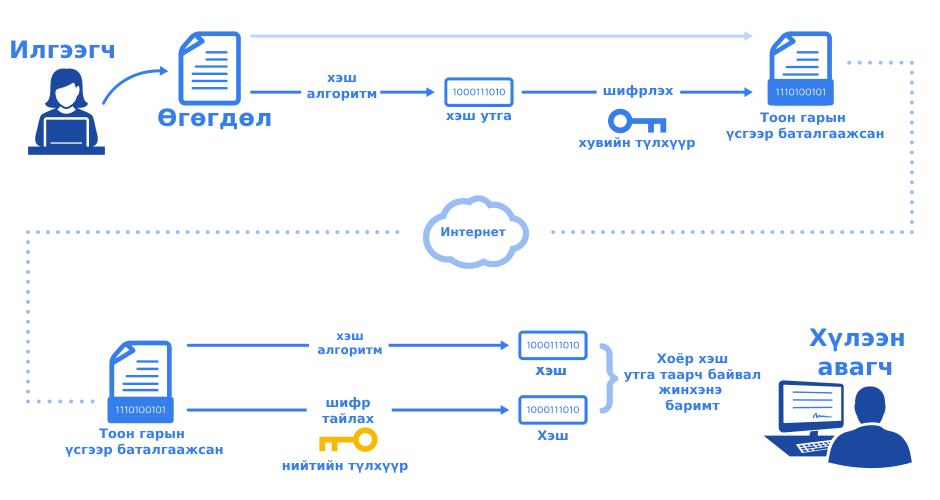
\includegraphics[scale=0.5]{assets/digisigi.png}
	\caption{Тоон гарын үсгийн ажиллах зарчим}
	\label{fig:architecture}
\end{figure}

\section{Адил системийн судалгаа}
\subsubsection{Tridumkey.mn}
Tridimkey нь Монгол улсын бүртгэлийн ерөнхий газраар хүлээн зөвшөөрөгдсөн тоон гарын үсэг олгогч ба байгуулагад зориулж гарын үсэг олгодог нь онцлог санагдсан.
Гэвч сул тал нь энэхүү тоон гарын үсгийн систем нь зөвхөн \textbf{Windows} үйлдлийн систем дээр ажилдаг ба Macos эсвэл Linux үйлдлийн систем ашигладаг хэрэглэгчид ашиглах боломжгүй болж байгаа юм.
\subsubsection{Monpass.mn}
Өөрсдийнх нь танилцуулгад "Таньж баталгаажуулах тоон гарын үсгийн гэрчилгээ: Цахим бизнес, төрийн болон бусад төрөл бүрийн систем, онлайн үйлчилгээнд хандах, бусад цахим гүйлгээ, хэлцэл хийхэд найдвартай таньж баталгаажуулах, захидал харилцааг хөдөлбөргүй баталгаажуулахын тулд тоон гарын үсэг зурах, захидал харилцаа, дамжуулж буй баримт бичгийг шифрлэн дамжуулах, ажилтнууд, хэрэглэгчдийг хялбар таних, бөөний онлайн худалдаа зохион байгуулах гэх мэт зорилгоор ашиглагддаг тоон гарын үсгийн гэрчилгээ – цахим баримт бичиг юм. Энэ гэрчилгээ нь хэрэглэгчийн мэдээлэл, олгосон ГОБ-ын мэдээлэл, хосгүй серийн дугаар болон бусад хосгүй өгөгдлүүд, хүчинтэй хугацаа, тоон гарын үсгийн нийтийн түлхүүр, холбогдох бусад мэдээллийг агуулсан байх бөгөөд Хувь хүмүүс болон байгууллагын төлөөлөгч хэн боловч ашиглаж болно. Захидал, мэдээлэлдээ тоон гарын үсэг зурахдаа өөрийн тоон гарын үсгийн хувийн түлхүүрийг ашиглах ба харин шифрлэн илгээх бол хүлээн авагчийн нийтийн түлхүүрийг ашиглана." гэсэн танилцуулагатай байсан ба гүнзгий судалж үзэхэд мөн л хэрэглэгчийн үйлдлийн систем зөвхөн \textbf{Windows} байж л тоон гарын үсгийн ашиглах боломжтой байсан юм.
\chapter{Системийн судалгаа, зохиомж}
\section{Үүлэн технологийн судалгаа}
Үүлэн технологи буюу үүлэн тооцоолол гэдэг нь өөрийн сервер эсвэл хувийн компьютерын оронд мэдээлэл хадгалах, удирдах, боловсруулах зорилгоор интернэтэд байрлах серверийн сүлжээг ашиглахын хэлж буй нэр томьёо юм.

Үүлэн технологийн хамгийн чухал давуу талуудын нэг нь өртөг багатай байдаг. Үүлэн технологийг ашигласнаар бизнесүүд өөрсдийн мэдээллийн технологийн дэд бүтцээ эзэмших, засвар үйлчилгээ хийх зэрэг урьдчилсан зардал, хүндрэлээс зайлсхийдэг ба зөвхөн ашигласан хэмжээнийхээ зардлыг л төлдөг. Өөр нэг гол давуу тал нь өндөр ачаалал даах уян хатан чанар бөгөөд бизнесүүд тооцоолох хэрэгцээгээ нэмэгдүүлэхийн хэрээр илүү их нөөцийг асар түргэн ашиглах эсвэл тооцоолох хэрэгцээ нь буурах тусам мөн хэрэгцээгээ танах боломжийг шууд олгодог.

Үүлэн технологи нь өгөгдөл сэргээх хадгалах шийдлүүдтэй бөгөөд энэ нь эмзэг мэдээллийг хадгалахад илүү найдвартай сонголт болдог. Хүртээмжтэй байдал нь бизнесүүдийг татдаг үүлэн технологийн бас нэг онцлог юм. Интернэт холболттой бол хэрэглэгчид дэлхийн хаанаас ч өгөгдөл, программдаа хандах боломжтой.

Үүлэн дээр суурилсан тоон гарын үсгийн үйлчилгээ нь хэрэглэгчдэд хүссэн үедээ ямар ч төхөөрөмжөөс баримт бичигт найдвартай гарын үсэг зурах, хадгалах, удирдах боломжийг олгох боломжтой. Энэхүү үйлчилгээ нь баримт бичигт гарын үсэг зурахад заавал биеэр очсон байх шаардлагагүй бөгөөд ингэснээр олон төрлийн үйл явцыг хялбаршуулах боломжтой. Өнөөгийн байдлаар энэ чиглэлд хамгийн томоохон үйлчилгээ үзүүлэгчид нь Amazon Web Services, Google Cloud Platform, Microsoft Azure зэрэг байна.

\pagebreak
\section{Системийн шаардлага}
\subsubsection{Функциональ шаардлагуудыг дараах хүснэгтэд тодорхойлов}
% table
\begin{table}[h]
	\centering
	\caption{Функциональ шаардлага}
	\begin{tabular}{ |p{2cm}|p{13cm}| }
		\hline
		ФШ 100 & Систем нь хэрэглэгчийн тоон гарын үсэг үүсгэх чадвартай байх ёстой. Үүнд хэрэглэгч бүрийн өвөрмөц түлхүүрийн хослолыг бий болгох орно.                                                                             \\ \hline
		ФШ 200 & Систем нь тоон гарын үсгийг баталгаажуулах функцээр хангах ёстой. Энэ нь гарын үсэг зурсан баримт бичгийг хүлээн авч, гарын үсэг зурсан хүний нийтийн түлхүүрийг ашиглан гарын үсгийг баталгаажуулах ёстой.        \\ \hline
		ФШ 300 & Систем нь хэрэглэгчдэд гарын үсэг зурахын тулд янз бүрийн форматтай цахим баримт бичгүүдийг (жишээлбэл, .doc, .pdf, .xls гэх мэт) байршуулахыг зөвшөөрөх ёстой.                                                    \\ \hline
		ФШ 400 & Систем нь хэрэглэгчдийг баримт бичигт гарын үсэг зурах, баталгаажуулахаас өмнө баталгаажуулах ёстой. Үүнийг хэрэглэгчийн нэр/нууц үг, олон хүчин зүйлийн баталгаажуулалт эсвэл бусад аюулгүй аргуудаар хийж болно. \\ \hline
		ФШ 500 & Систем нь баримт бичиг байршуулах, гарын үсэг үүсгэх, гарын үсгийн баталгаажуулалт зэрэг хэрэглэгчдийн хийсэн бүх үйлдлийг бүртгэх ёстой.                                                                          \\ \hline
		ФШ 600 & Систем нь бусад үйлчилгээтэй нэгтгэх API-г өгөх ёстой. Энэ нь бусад программ хангамж эсвэл үйлчилгээнд энэ үйлчилгээний тоон гарын үсгийн чадварыг ашиглах боломжийг олгоно.                                        \\  \hline

	\end{tabular}
\end{table}
\pagebreak
\subsubsection{Функциональ бус шаардлагуудыг дараах хүснэгтэд тодорхойлов}
% table
\begin{table}[h!]
	\centering
	\caption{Функциональ бус шаардлага}
	\begin{tabular}{ |p{2cm}|p{13cm}| }
		\hline
		ФБШ 100 & Систем нь GDPR эсвэл HIPAA гэх мэт холбогдох бүх мэдээллийн аюулгүй байдал, нууцлалын дүрэм журмыг дагаж мөрдөх ёстой. Гарын үсэг, баримт бичиг зэрэг бүх өгөгдөл шифрлэгдсэн байх ёстой. \\ \hline
		ФБШ 200 & Систем нь гүйцэтгэлийн бууралтгүйгээр олон тооны хэрэглэгчид болон баримт бичгүүдийг зохицуулах чадвартай байх ёстой.                                                                     \\ \hline
		ФБШ 300 & Үүлэн үйлчилгээ нь хамгийн бага зогсолттой, 24/7 цагийн турш ашиглах боломжтой байх ёстой. Үйлчилгээний түвшний гэрээ (SLA) нь дор хаяж 99.9\% ажиллах хугацааг баталгаажуулах ёстой.     \\ \hline
		ФБШ 400 & Систем нь хүлээн зөвшөөрөгдсөн тодорхой хугацааны дотор гарын үсэг үүсгэх, баталгаажуулах хүсэлтийг хурдан боловсруулах чадвартай байх ёстой.                                             \\ \hline
		ФБШ 500 & Систем нь янз бүрийн техникийн чадвартай хэрэглэгчдэд үүнийг үр дүнтэй ашиглах боломжийг олгодог хэрэглэгчдэд ээлтэй интерфэйстэй байх ёстой.                                             \\ \hline
		ФБШ 600 & Үүлэн үйлчилгээ нь янз бүрийн үйлдлийн систем, хөтөч, төхөөрөмжтэй нийцтэй байх ёстой.                                                                                                    \\  \hline
		ФБШ 700 & Энэ систем нь гамшгийн үед өгөгдөл алдагдахгүй байхын тулд найдвартай нөөцлөх, сэргээх механизмтай байх ёстой.                                                                            \\ \hline
		ФБШ 800 & Систем нь Европ дахь eIDAS эсвэл АНУ-ын ESIGN хууль зэрэг тоон гарын үсгийн хууль тогтоомж, дүрэм журамд нийцсэн байх ёстой.                                                              \\ \hline
	\end{tabular}
\end{table}
\newpage

\section{Use case диаграм}
\begin{figure}[h]
	\centering
	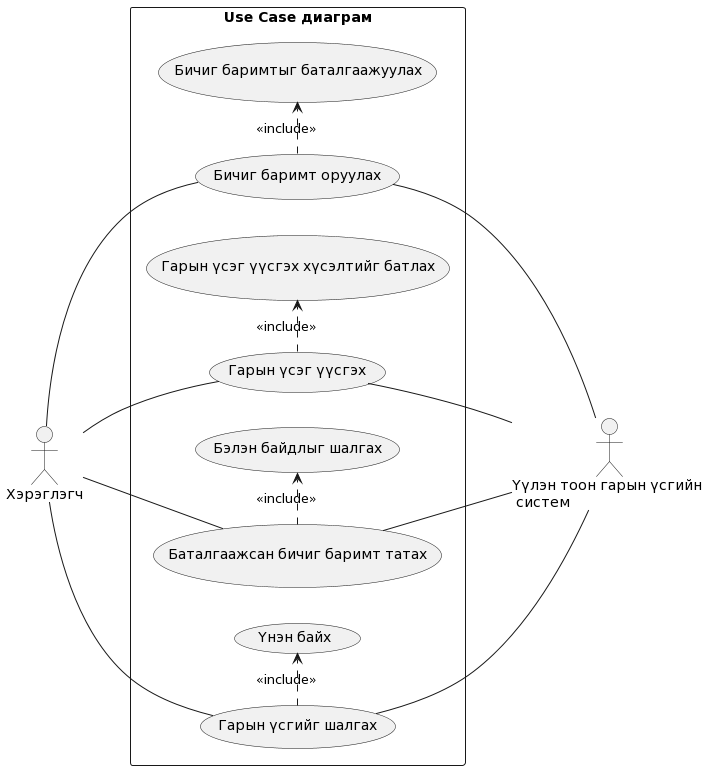
\includegraphics[scale=0.66]{assets/usecase_mn.png}
	\caption{Use case диаграм}
	\label{fig:usecasemn}
\end{figure}
\begin{enumerate}
	\item Хэрэглэгч системийг ашиглан өөрийн бичиг баримтыг зурахын тулд эхлээд эдгээр баримтын систем рүү оруулж өгсөн байх шаардлагатай.
	\item Хэрэглэгч өөрийн гарын үсгийг үүсгэх эсвэл, хүний оролцоогүй системээр автоматаар үүсгүүлэх боломжтой.
	\item Хэрэглэгч баталгаажсан бичиг баримтыг гурав хоногийн дотор татаж авах боломжтой.
\end{enumerate}
\pagebreak
\section[Sequence диаграм]{Хэрэглэгч баримт баталгаажуулах sequence диаграммыг харуулав}
\begin{figure}[h!]
	\centering
	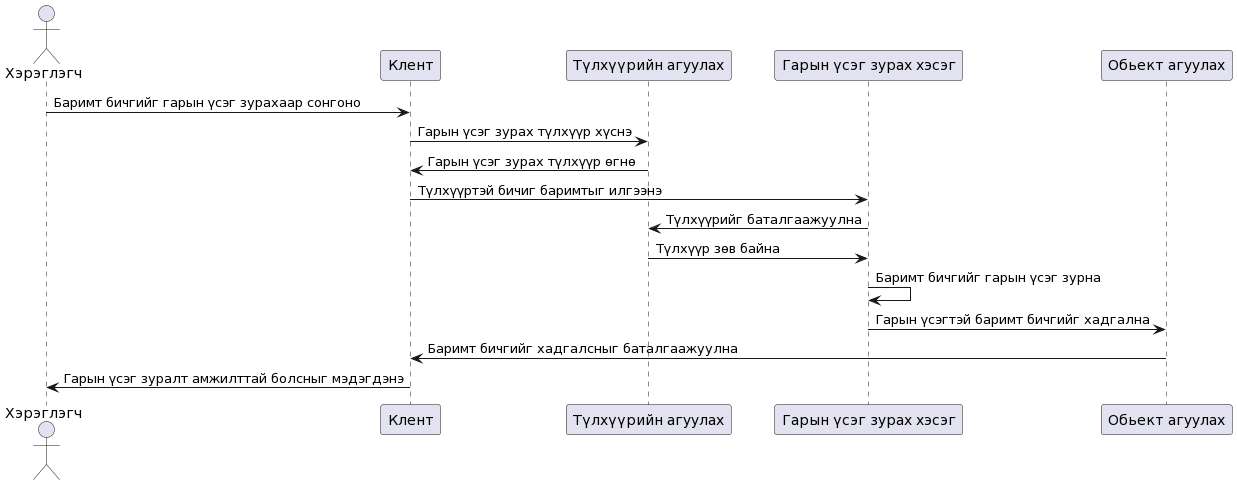
\includegraphics[scale=0.45, angle=90]{assets/sequence2.png}
	\caption{Sequence диаграм}
	\label{fig:usecasemn}
\end{figure}
\newpage
\section[ӨС диаграм]{Өгөгдлийн сангийн диаграм}

\begin{figure}[h!]
	\centering
	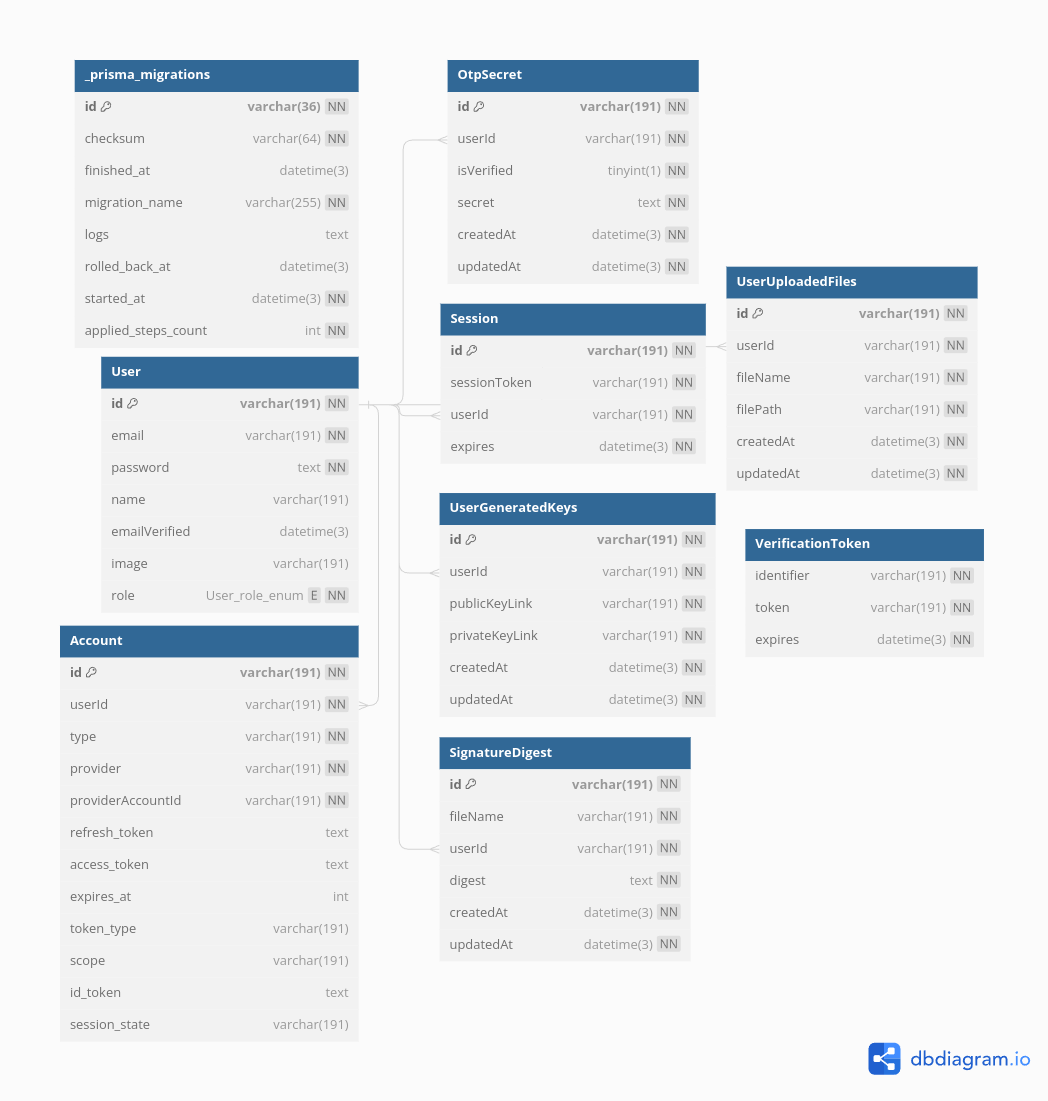
\includegraphics[scale=0.5]{assets/cryptography.png}
	\caption{Өгөгдлийн сангийн диаграм}
	\label{fig:dbdiagram}
\end{figure}
\break
\newpage
\section{Архитектур}
Энэхүү төслийг ажиллахад илүү хямд зардалтай хүртээмжтэй, ачаалал даах чадварыг нэмэх зорилгоор серверлесс Архитектур сонгосон юм. Фронт-энд хэсэг нь NextJS-н ашигласан тул Сервер талын рендер хийж байгаа ба Бак-энд хэсэг нь тэр чигтээ AWS-н Ламдба функц дээр ажиллах юм. Хэрэглэгчийн серверлүү илгээж байгаа бичиг баримтыг AWS-н Ламдба дээр үүсгэсэн нэг удаагийн холбоосоор хэрэглэгч шууд AWS-руу оруулах юм. Өмнө нь Whatsapp ийм маягаар файл оруулдаг байсан жишээнээс санаа авсан. Статик файлуудыг AWS-н Cloud Front дээр байрлуулсан ба энэ нь дэлхийн өнцөг бүрт байдаг хэрэглэгчид хамгийн ойрхан контент түгээх сүлжээ юм энэ нь хэрэглэгчид илүү хурдан татах боломжийг олгохоос гадна мөн сагхүүгийн хувьд хэмнэлттэй болдог юм. Хэт их хэмжээний хандалт, халдлага зэргээс сэргийлэх зорилгоор AWS-WAF ашиглаж бүх хүсэлтүүд илгээгдэнэ.
\begin{figure}[h!]
	\centering
	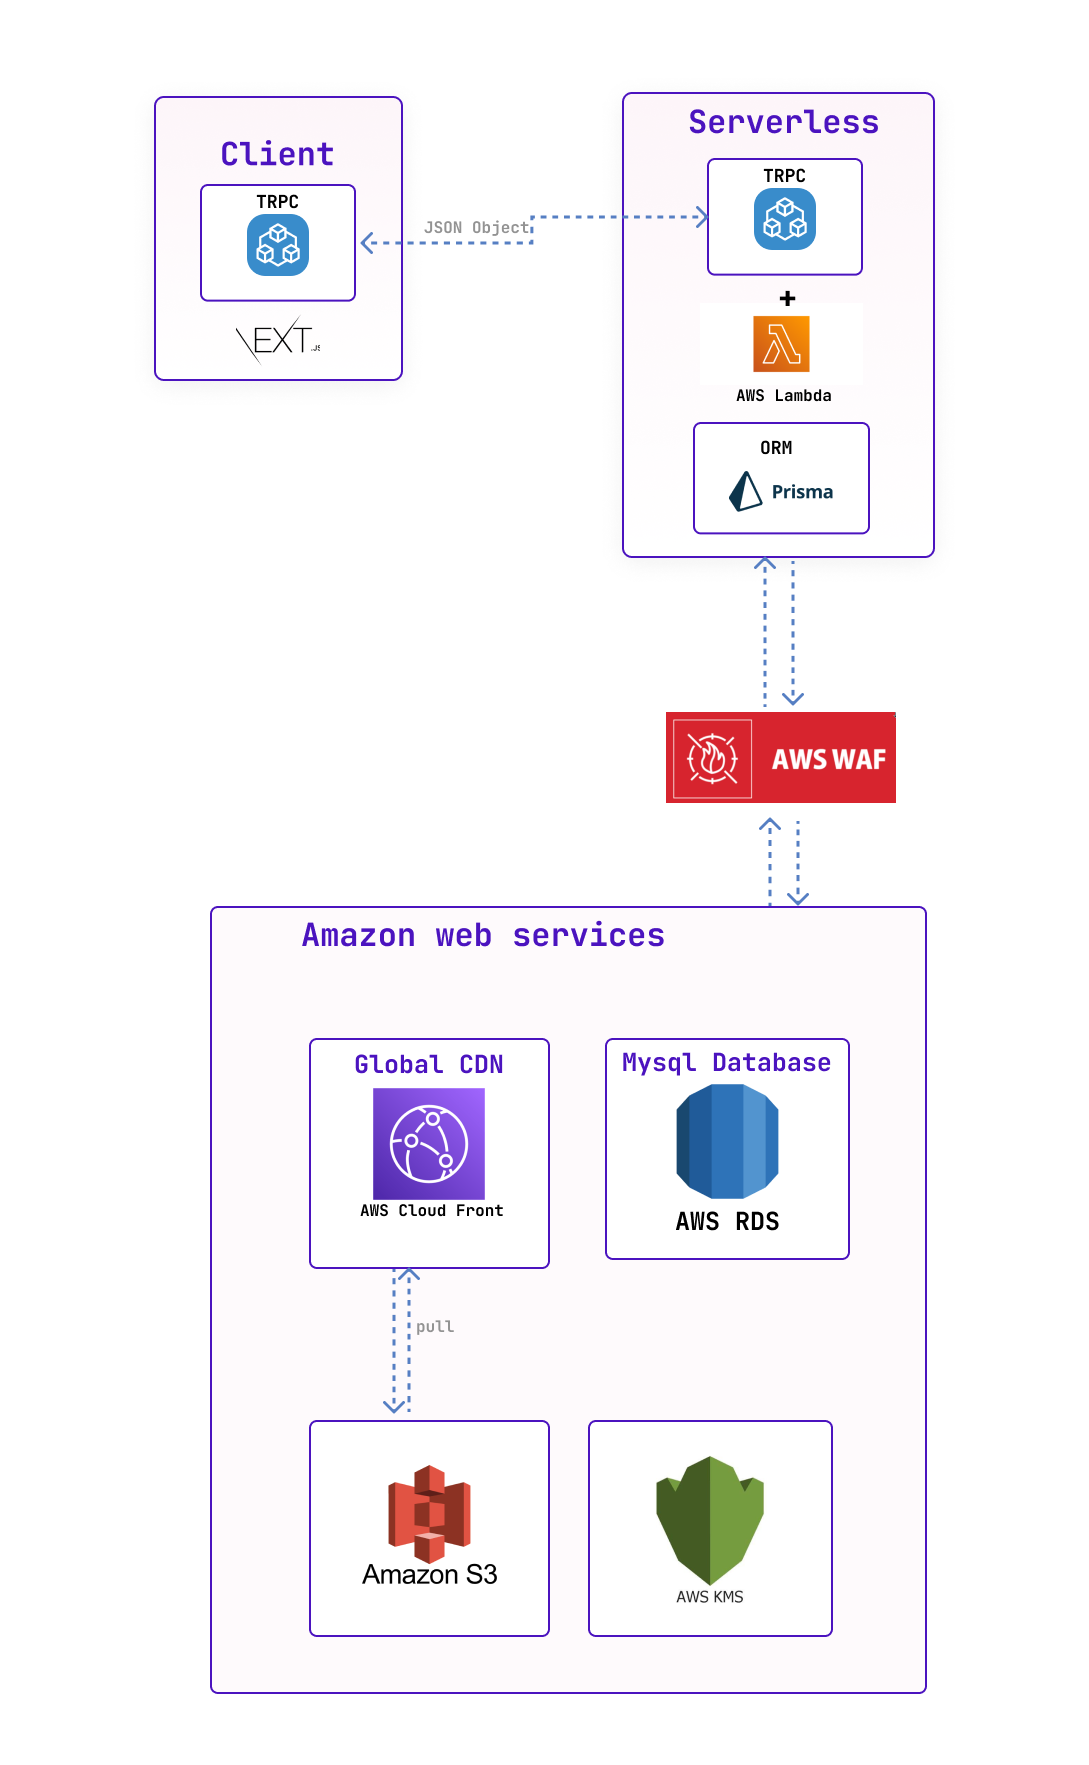
\includegraphics[scale=0.32]{assets/server.png}
	\caption{Архитектурын зураг}
	\label{fig:architecture}
\end{figure}
\pagebreak
\newpage
\section[ӨС хүснэгтүүд]{Өгөгдлийн сангийн хүснэгтүүд}

\begin{table}[h]
	\caption{User хүснэгт}
	\begin{tabular}{|l|l|l|p{8cm}|}
	\hline
	№ &  Талбарын нэр & Өгөгдлийн төрөл & Тайлбар \\ \hline
	1 &  id & Varchar & Хэрэглэгчийн дахин давтагдашгүй ID-г хад-
	гална\\ \hline
	2 &  email & Varchar & Хэрэглэгчийн цахим шууданг хадгална\\ \hline
	3 &  password & Varchar & Хэрэглэгчийн нууц үгийг шифрлэж, энэ талбарт хадгална \\ \hline
    4 &  name & Varchar & Хэрэглэгчийн интерфейсээс оруулсан хэрэглэгчийн нэр. Зөвхөн латин үсгийг хадгална. \\ \hline
	5 &  emailVerified & DateTime & Хэрэглэгчийн имэйлийг баталгаажуулсан цагийн тэмдэ \\ \hline
	6 &  image & Varchar & Хэрэглэгчийн байршуулсан зургийн холбоос хадгалагдах бөгөөд зам нь энэ талбарт хадгалагдана \\ \hline
\end{tabular}
\end{table}

\begin{table}[h]
	\caption{Session хүснэгт}
	\begin{tabular}{|l|l|l|p{8cm}|}
	\hline
	№ &  Талбарын нэр & Өгөгдлийн төрөл & Тайлбар \\ \hline
	1 &  id & Varchar & Нэвтрэлтийн түүхийн өвөрмөц ID \\ \hline
	2 &  sessionToken & Varchar & Гуравдагч этгээдийн токен (Github, Google) байна. \\ \hline
	3 &  userId & Varchar & Хэрэглэгчийн өвөрмөц ID \\ \hline
	4 &  expires & DateTime & Дуусах хугацаа \\ \hline
\end{tabular}
\end{table}

\begin{table}[h]
	\caption{UserGeneratedKeys хүснэгт}
	\begin{tabular}{|l|l|l|p{8cm}|}
	\hline
	№ &  Талбарын нэр & Өгөгдлийн төрөл & Тайлбар \\ \hline
	1 &  id & Varchar & Өвөрмөц ID\\ \hline
	2 &  userId & Varchar & Түлхүүрийг үүсгэсэн хэрэглэгчийн ID \\ \hline
	3 &  publicKeyLink & Varchar & Нийтийн түлхүүрийн байршил \\ \hline
	4 &  privateKeyLink & Varchar & Хувийн түлхүүрийн байршил \\ \hline
	5 &  createdAt & DateTime & Үүсгэсэн огноо \\ \hline
	6 &  updatedAt & DateTime & Шинэчилсэн огноо \\ \hline
\end{tabular}
\end{table}
\begin{table}[h]
	\caption{VerificationToken хүснэгт}
	\begin{tabular}{|l|l|l|p{8cm}|}
	\hline
	№ &  Талбарын нэр & Өгөгдлийн төрөл & Тайлбар \\ \hline
	1 &  identifier & Varchar & Токенд зориулсан өвөрмөц ID\\ \hline
	2 &  token & Varchar & Баталгаажуулалтын Токен \\ \hline
	3 &  expires & DateTime & Дуусах хугацаа \\ \hline
\end{tabular}
\end{table}

\begin{table}[h]
	\caption{Account хүснэгт}
	\begin{tabular}{|l|l|l|p{8cm}|}
	\hline
	№ &  Талбарын нэр & Өгөгдлийн төрөл & Тайлбар \\ \hline
	1 &  id & Varchar & Өвөрмрц ID \\ \hline
	2 &  userId & Varchar & Энэ бүртгэлтэй холбоотой хэрэглэгчийн ID \\ \hline
	3 &  type & Varchar & Бүртгэлийн тө \\ \hline
	4 &  provider & Varchar & Аль гуравдагч этгээдийг дамжиж нэвтэрсэн (Github, Google) \\ \hline
	5 &  providerAccountId & Varchar & Хаягийн өвөрмөц ID \\ \hline
    6 &  refresh\_token & Varchar & Шинэ токен үүсгэх нууц үг\\ \hline
    7 &  access\_token & Varchar & Баталгаажуулах токен \\ \hline
    8 &  expires\_at & Int & Дуусах хугацаа\\ \hline
    9 &  token\_type & Varchar & Төрөл \\ \hline
    10 &  scope & Varchar & Нэвтрэлтийн эрх \\ \hline
    11 &  id\_token & Varchar & Өвөрмөц ID \\ \hline
    12 &  session\_state & Varchar & Одоо нэвтрэлттэй байгаа эсэх\\ \hline
\end{tabular}
\end{table}

\begin{table}[h]
	\caption{UserUploadedFiles хүснэгт}
	\begin{tabular}{|l|l|l|p{8cm}|}
	\hline
	№ &  Талбарын нэр & Өгөгдлийн төрөл & Тайлбар \\ \hline
	1 &  id & Varchar & Хэрэгдэгчийн оруулсан файлын өвөрмөц ID\\ \hline
	2 &  userId & Varchar & Файлыг байршуулсан хэрэглэгчийн ID \\ \hline
	3 &  fileName & Varchar & Файлын нэр\\ \hline
	4 &  filePath & Varchar & Файл хадгалагдаж буй зам \\ \hline
	5 &  createdAt & DateTime & Файлыг байршуулсан цаг \\ \hline
	6 &  updatedAt & DateTime & Файлын мэдээлэл хамгийн сүүлд шинэчлэгдсэн цаг \\ \hline
\end{tabular}
\end{table}

\begin{table}[h]
	\caption{OtpSecret хүснэгт}
	\begin{tabular}{|l|l|l|p{8cm}|}
	\hline
	№ &  Талбарын нэр & Өгөгдлийн төрөл & Тайлбар \\ \hline
	1 &  id & Varchar & Нэг удаагийн нууц үг үүсгэх түлхүүрийн ID\\ \hline
	2 &  userId & Varchar & Холбоотой хэрэглэгчийн ID \\ \hline
	3 &  isVerified & Boolean & OTP нь баталгаажсан эсэх \\ \hline
	4 &  secret & Text & Нэг удаагийн нууц үгийн баталгаажуулалтад ашигласан нууц \\ \hline
	5 &  createdAt & DateTime & OTP үүсгэсэн цаг\\ \hline
	6 &  updatedAt & DateTime & Хамгийн сүүлд шинэчилсэн цаг\\ \hline
\end{tabular}
\end{table}

\begin{table}[h]
	\caption{SignatureDigest хүснэгт}
	\begin{tabular}{|l|l|l|p{8cm}|}
	\hline
	№ &  Талбарын нэр & Өгөгдлийн төрөл & Тайлбар \\ \hline
	1 &  id & Varchar & Нууц үгийн хайшийн ID\\ \hline
	2 &  fileName & Varchar & Холбогдсон файлын нэр \\ \hline
	3 &  userId & Varchar & Харгалзах хэрэглэгчийн ID\\ \hline
	4 &  digest & Text & Хайшын утга \\ \hline
	5 &  createdAt & DateTime & Үүсгэсэн огноо \\ \hline
	6 &  updatedAt & DateTime & Шинэчилсэн огноо \\ \hline
\end{tabular}
\end{table}

\pagebreak
\newpage


\chapter{Хэрэгжүүлэлт}
\section{Сонгосон технологи}
\subsection{Nextjs \& Reactjs}
\subsubsection{Declarative}
React нь хэрэглэгчийн интерактив интерфейс бүтээхийг хялбарчилдаг. Aппликейшны state бүрд зориулсан энгийн бүтэц зохион байгуулахаас гадна, React нь өгөгдөл өөрчлөгдөхөд яг зөв компонентоо өөрчлөн рендер хийдэг. Declarative бүтэц нь кодыг тань debug хийхэд хялбар болгохоос гадна, ажиллагаа нь илүү тодорхой болдог

\subsubsection{Компонент-д тулгуурласан}
Бие даан state-ээ удирддаг маш энгийн компонент бичиж, эдгээрийг хольж найруулан нарийн бүтэцтэй хэрэглэгчийн интерфейс бүтээ.

Компонентийн логик нь тэмплэйт-ээр бус JavaScript-ээр бичигддэг учраас өгөгдлийг апп хооронд хялбар дамжуулж, DOM-оос state-ээ тусд нь байлгаж чадна.

\subsubsection{Nextjs}
Netflix, TikTok, Hulu, Twitch, Nike гэсэн орчин үеийн аваргууд ашигладаг энэхүү орчин үеийн фрэймворк нь React технологи дээр үндэслэгдсэн бөгөөд Frontend Backend хоёр талд хоёуланд нь ажилладаг веб аппуудыг хийх чадвартайгаараа бусдаасаа давуу юм. Next.js -ийн үндсэн дизайн нь клиент болон сервер талын аль алиных давуу талыг ашиглаж чаддаг, ямар нэг дутагдалгүй веб сайтыг яаж хамгийн хурдан хялбар бүтээх вэ гэдгийг бодож тусгасан байдаг. Next.js нь сервер талд react компонентуудыг рендерлэн энгийн html, css, json файл болгон хувиргах замаар ажилладаг бөгөөд 2020 оноос олон нийтэд танигдсан JAMStack технологи болон статик сайт, автоматаар статик хуудас үүсгэх, CDN deployment, сервергүй функц, тэг тохиргоо, файлын системийн рүүтинг (PHP-ээс санаа авсан), SWR (stale while revalidate), сервер талд рендерлэх зэрэг асар олон орчин үеийн шинэхэн технологиудыг бүгдийг хийж чаддаг анхны бүрэн веб фрэймворк гэж хэлж болно.\cite{Reactjs}
\subsection{tRPC (Back End)}

Энгийнээр хэлбэл, tRPC нь клиент болон сервер хоорондоо сүлжээгээр харилцаж болох API (Application Programming Interfaces) бүтээх хэрэгсэл юм. Энэ нь хувьсагчийн төрлүүдийг нягт зааж өгч Front-End Back-End хоёрийг холбож ажилладаг. Жишээ нь хэрвээ сервер тал дээр ажиллаж байгаа хөгжүүлэгч, функцын параметр солиход энгийн REST api эсвэл Graphql түүнийг мэдэж чадахгүй юм. Харин tRPC нь шууд алдаа болж харагдах ба хөгжүүлэлтийн орчинд Back-end Front-end хоёр холбогдож ажилдаг гэдгээрээ давуу юм. Ингэснээр хөгжүүлэхэд илүү хялбар, инжинерт илүү ээлтэй болдог билээ.
Кодыг \ref{lst:docker-compose}
\subsection{AWS S3 объект агуулах}
AWS S3 (Amazon Simple Storage Service) нь Amazon Web Services (AWS) дээрх өгөгдөл, мэдээллийг онлайнаар нөөцлөх, архивлахад зориулагдсан хязгааргүй өргөтгөх боломжтой, өндөр хурдтай, вэб технологит суурилсан үүлэн хадгалах үйлчилгээ юм. Энэ нь вэбийн хаанаас ч хүссэн үедээ ямар ч хэмжээний өгөгдлийг хадгалах, сэргээхэд ашиглаж болно.
\subsection{AWS KMS}
AWS Түлхүүр Удирдлагын Үйлчилгээ (KMS) нь криптографын түлхүүрүүдийг үүсгэх, хянахад хялбар болгодог. Мөн түүнчлэн түлхүүр нь ашиглагдаагүй хадгалагдаж байх үедээ шифрлэгдсэн байдаг.
Энэхүү үйлчилгээ нь бусад AWS үйлчилгээнүүдтэй нэгтгэгдсэн тул эдгээр үйлчилгээнд хадгалсан өгөгдлийг шифрлэх, кодыг тайлах түлхүүрүүдэд хандах хандалтыг хянахад хялбар болгодог.

\subsection{Dockerizing}
Орчин үеийн нэгэн гайхалтай технологи бол контайнерчлах юм. Яагаад Docker чухал вэ гэвэл, ямар нэгэн систем хөгжүүлэгчийн компьютер аль эсвэл ямар сервер дээр ажиллаж байгаагаас үл хамааран проргам нь өөрийн тусдаа орчинд ажиллах юм. Яг л Virtual machine шиг гэхдээ давуу тал нь Docker host system-ийнхээ цөмийг (kernel)-г ашигладаг учраас маш бага хэмжээгий зай, нөөц ашигладаг.
\subsection{CI/CD}
Мөн сүүлийн үед маш их өргөн түгж байгаа ойлголт бол Continuous Integration/Continuous Deployment.
Энэ нь проргам хангамж ямар ч нөхцөлд хөгжүүлэлт тасралтгүй явж байх орчноор хангадаг ба системд хэзээ ч тасалдал үүсгэхгүй мөн хүний оролцоог маш бага байлгах давуу талтай.\footnote{Дадлагын ажлаасаа иш татав. https://github.com/b4ljk/internship-report}.

\section{Ажиллагаа}
\subsection{Гарын үсэг зурах}
\subsubsection{Сервер талд ажиллах}
\begin{enumerate}
	\item Хэрэглэгчийн оруулсан файлыг объект агуулахаас (AWS S3) татаж авах.
	\item Файлын бинари (binary) хэсгийг SHA256 алгоритм ашиглан хайш утгыг тооцоолох.
	\item Хэрэглэгчийн хувийн түлхүүрийг аюулгүй хадгалах орчноос авах (AWS KMS).
	\item Хувийн түлхүүрийг ашиглах хайш утгыг шифрлэх.
	\item Шифрлэгдсэн утгыг өгөгдлийг сан руу хадгалах.
	\item Шифрлэгдсэн утга буюу гарын үсгийг олон улсын стандартын дагуу PDF файл руу нэмэх.
	\item Шинээр үүссэн буюу шифрлэгдсэн файлыг объект агуулах руу хуулах.
	\item Нэг удаагийн татаж авах холбоосыг хэрэглэгчид өгөх.
\end{enumerate}
\subsubsection{Хэрэглэгч талд ажиллах}
\begin{enumerate}
	\item Хэрэглэгчийн өөрийн файлыг оруулах.
	\item Файлын бинари (binary) хэсгийг SHA256 алгоритм ашиглан хайш утгыг тооцоолох.
	\item Хэрэглэгч хувийн түлхүүрээ оруулах.
	\item Хувийн түлхүүрийг ашиглах хайш утгыг шифрлэх.
	\item Шифрлэгдсэн утгыг сервер рүү илгээх.
	\item Шифрлэгдсэн утга буюу гарын үсгийг олон улсын стандартын дагуу PDF файл руу нэмэх.
	\item Хэрэглэгч талд гарын үсэг зурсан файл үүсэх.
\end{enumerate}

\section{Хөгжүүлэлт}

\subsection{Хөгжүүлэлтийн орчныг бэлдэх}
Миний хувьд хөгжүүлэлтийн орчныг бэлдсэнээр нийт ажлын тал нь дуусдаг. Энэхүү судалгааны ажлын практик хэсэгт би NextJS, tRPC, PrismaORM, PlanetscaleDB, AWS зэргийг ашиглан хөгжүүлэлт хийх билээ. NextJS нь монолитик төсөл хийхэд тохиромжтой ба би төслийн сервер, клайнт талуудыг нэг repository-д хадгалж байгаа юмаа. Version Control System дээр Github-г соногосон юм. Кодын фолдер бүтэцmai нь дараах байдлаар байна.

\begin{figure}[h]
	\centering
	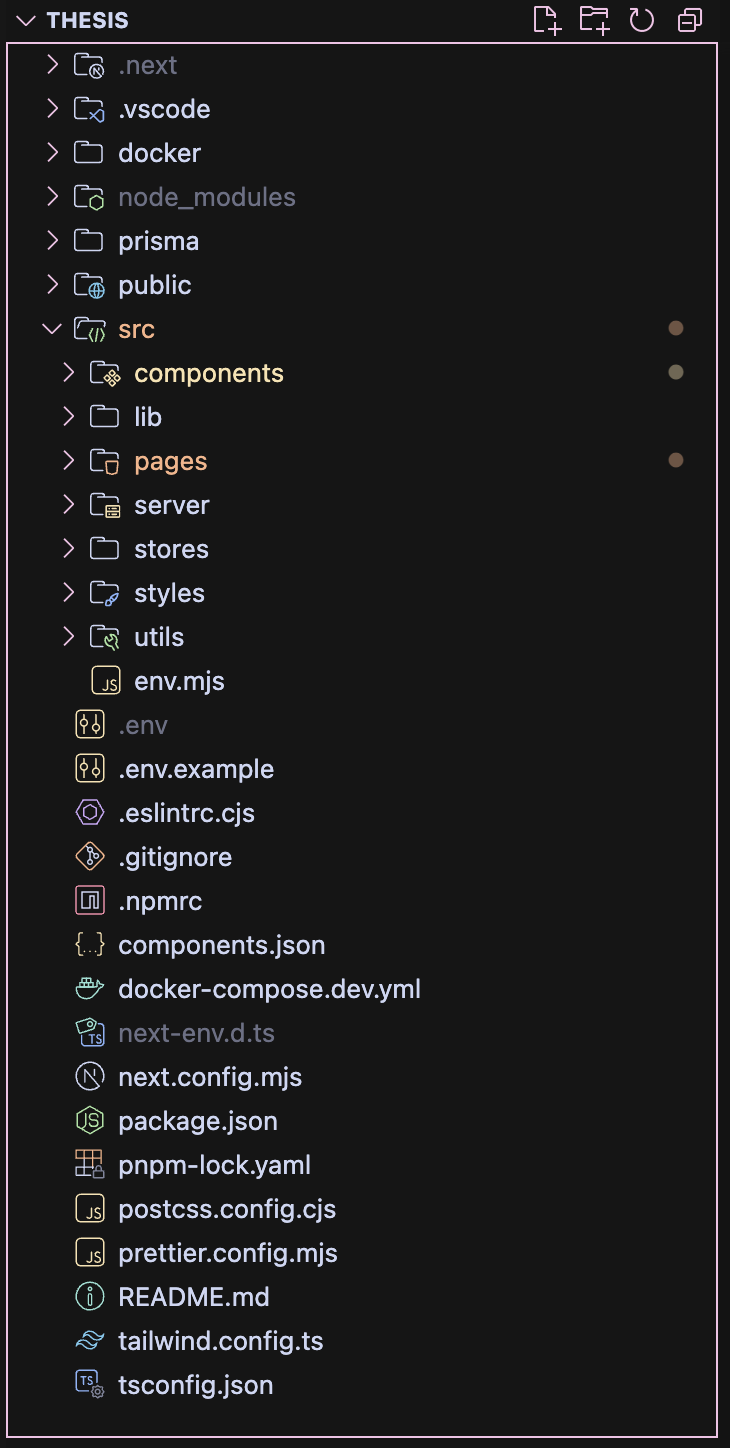
\includegraphics[scale=0.55]{assets/web/structure.png}
	\caption{Фолдерийн бүтэц}
	\label{fig:architecture}
\end{figure}
\begin{itemize}
	\item \textbf{.github/workflows} - CI/CD хийхэд шаардлагатай файлууд
	\item \textbf{components} - React компонентууд
	\item \textbf{lib} - Хэрэглэгчийн талын шаардлагатай код туслах функцууд
	\item \textbf{pages} - NextJS дээрх хуудаснууд
	\item \textbf{prisma} - Prisma ORM-ийн өгөгдлийн сангийн зохион байгуулалт
	\item \textbf{public} - Хуудаснуудын зураг, css файлууд
	\item \textbf{server} - Сервер талын код
	\item \textbf{store} - Хэрэглэгчийн талын төлвийг (state) хадгалах сан
	\item \textbf{docker} - Dockerfile, docker-compose файлууд
\end{itemize}

\subsubsection{Өгөгдлийн сангийн зохион байгуулалт}
Призма нь өгөгдлийн сан болон, код баз хоёрын хялбараар холбоход тусладаг. Үүнийг ORM гэж нэрлэдэг ба давуу тал нь, өгөгдлийг ариутгах, өгөгдлийг сангийн зохион байгуулалт түүхийг хадгалах зэрэг ажлыг инжинер хийх шаардлаггүй болох юм.
\lstinputlisting[language=Typescript,lastline=30, caption=Prisma Датабаазын модел,label=lst:prisma,frame=single]{src/code/schema.prisma}

\subsubsection{AWS}
Амазоны санал болгодог үйлчилгээнүүдийг өөртөө тохирхийг нь ашигласнаар заавал өөрийн серверийг ажлуулах шаардлаггүй болно. Мэдээж ашиглахийн тулд AWS дээрээ тохиргоонуудыг хийх ба нууцлалын мэдээллүүдээ код дундаа оруулж үүнийгээ ашиглах юм.

Жишээ нь хэрэглэгчийн оруулсан файлыг 3 хоногийн дараа устана гэсэн тохиргоог AWS дээр хийж өгсөн байгаа.

\lstinputlisting[language=Typescript, caption=AWS нууцлалын хэсэг,label=lst:aws,frame=single]{src/code/aws.ts}

\lstinputlisting[language=Typescript,lastline=51, caption=Файл серверлүү урсгалаар илгээх,label=lst:stream,frame=single]{src/code/awsHelper.ts}

\subsubsection[Front-end]{Хэрэглэгчийн хэсгийн хөгжүүлэлт (Front-end)}
Энэ хэсэгт хэрэглэгчийн сервертэй харьцах API хэсэг хийгдсэн ба tRPC нь хэрэглэгчийн талаас серверлүү хүсэлт илгээхдээ хүүк бичих байдлаар ажилдаг. Доор оруулсан код нь  API-тэй холбоотойгоор ямар нэгэн алдаа гарвал вэб аппликейшныг тэр чигт нь унагахгүйгээр ямар ч алдааг хэрэглэгчид ойлгомжтой мессеж болгож харуулах код.
\lstinputlisting[language=Typescript,firstline=32,lastline=58, caption=Глобал алдааны мэдээллэгч,label=lst:stream,frame=single]{src/code/api.ts}

\subsubsection[Back-end]{Сервер хэсгийн хөгжүүлэлт (Back-end)}
Middleware нь кодыг эмх цэгцтэй байхад хэрэг болдог ба хэрэглэгчээс хүсэлт ирэхэд сервер хариу өгөхийн яг өмнөхөн ажилдаг хэсэг код билээ. Энэ хэсэгт хэрэглэгчийн мэдээллийг шалгах, нэвтэрсэн үгүйг тодорхойлох зэргийг хийхэд тохиромжтой байдаг.
\lstinputlisting[language=Typescript,firstline=49,lastline=62, caption=Middleware,label=lst:Middleware,frame=single]{src/code/trpc.ts}
Бүх API нь нэгдсэн байдлаар нэг газар зангидагдаж байх ёстой. Миний хувьд tRPC дээрх бүх API-г root.ts гэдэг файл дотор нэгтгэж сервэрийн кодны үндэс болгож байгаа юм.
\lstinputlisting[language=Typescript, caption=Root,label=lst:Root,frame=single]{src/code/root.ts}

\section{РСА (RSA) Хэрэгжүүлэлт}
РСА нь $p$, ба  $q$ хоёр анхны тооны үржигдэхүүнээр $N$ буюу модулус тодорхойлогддог. Гэвч 2048 бит мэтийн маш их олон оронтой тоог анхны тоо эсэхийг нь шалгахад нүсэр тооцоолол орох болдог. Иймд Миллер-Рабины тестийг ашиглаж магадлалаар (probabilistic) анхны тоо эсэхийг нь мэддэг юм.


\lstinputlisting[language=Typescript,firstline=60,lastline=85, caption=RSA хэрэгжүүлэлт=lst:RSA,frame=single]{src/code/rsa.tsx}

Хэдий магадлалаар тооцож байгаа ч $k$ давталтаас хамаарч анхны тоо бус байх магадлал буурна. Жишээ нь $k = 10$ үед $\left(\frac{1}{4}\right)^{10}$ буюу саяд нэг байх магадлалтай байна.

\lstinputlisting[language=Typescript,firstline=16,lastline=48, caption=Миллер-Рабины тест=lst:RSA,frame=single]{src/code/rsa.tsx}



\section{Үр дүн}
Төслийн практик ажлын үр дүнд бүтээгдсэн үүлэн тоон гарын үсгийг системийн интерфейс дараах байдлаар харагдана.
\begin{figure}[h]
	\centering
	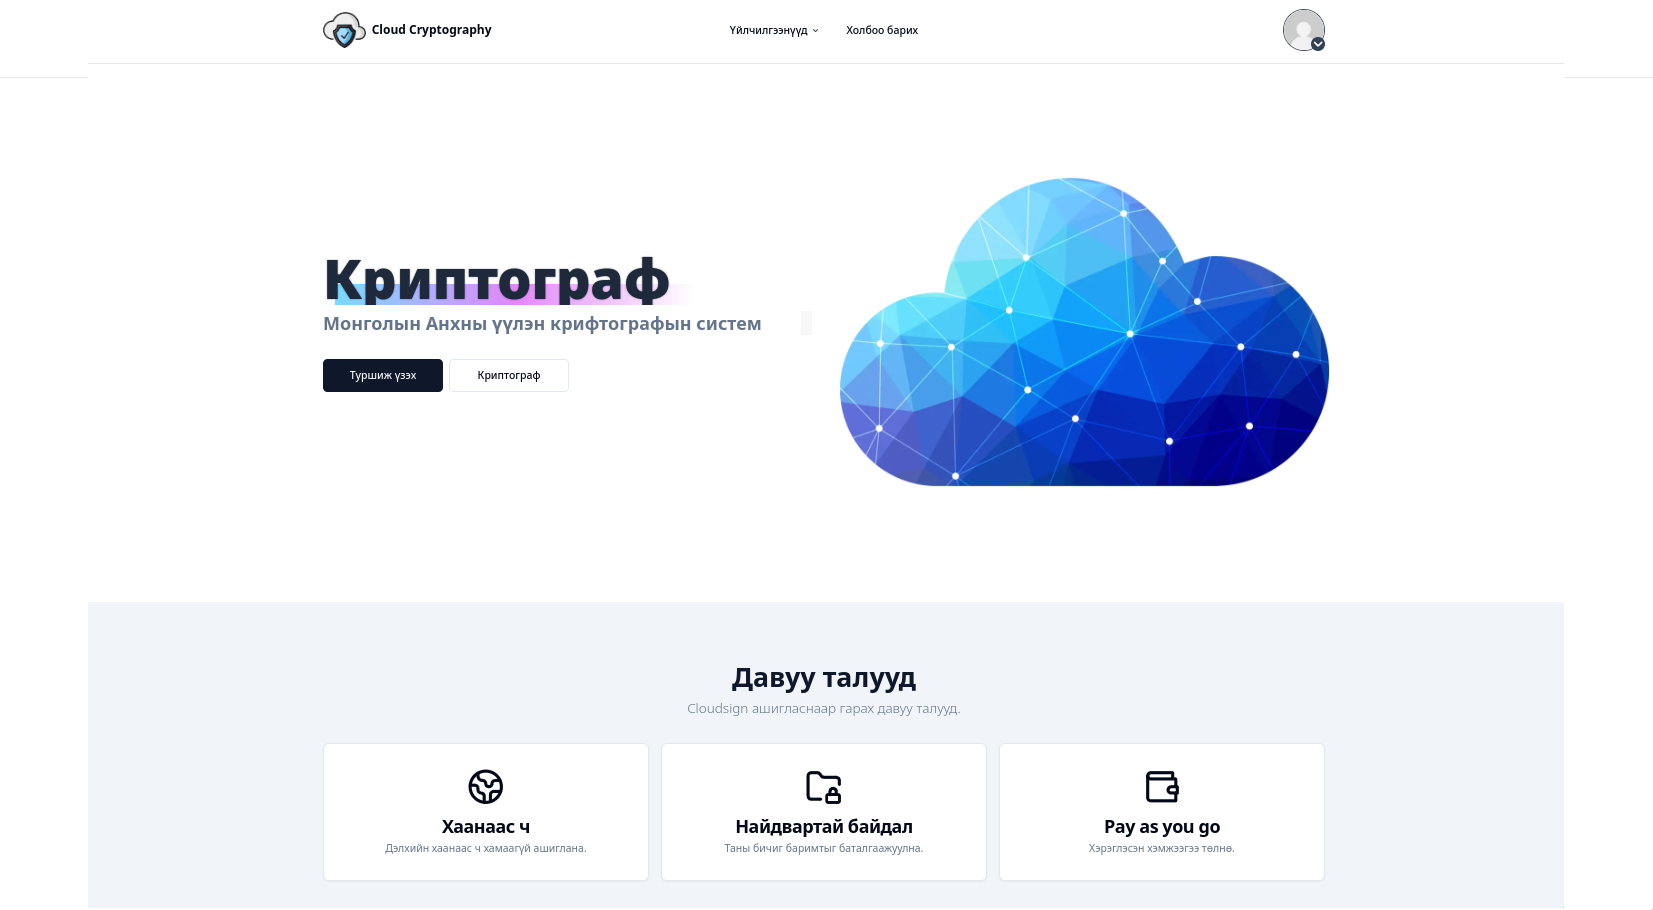
\includegraphics[scale=0.26]{assets/web/hero.png}
	\caption{Нүүр хуудас}
	\label{fig:architecture}
\end{figure}
\begin{figure}[h]
	\centering
	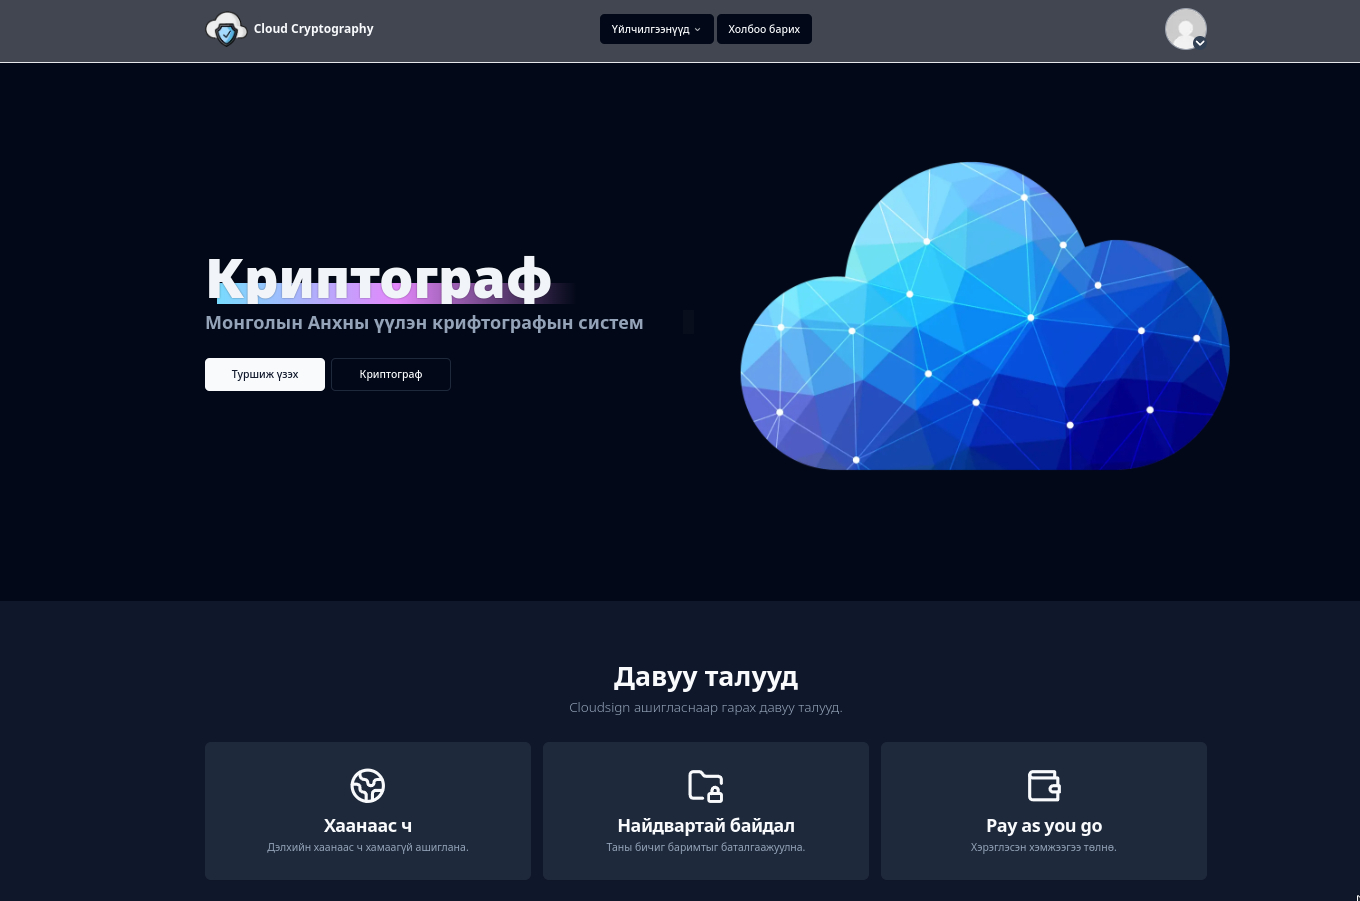
\includegraphics[scale=0.3]{assets/web/darkhero.png}
	\caption{Нүүр хуудас, Шөнийн тохиргоо}
	\label{fig:architecture}
\end{figure}
Өөрийн хувийн нийтийн түлхүүрийг, нууц үгтэйгээр үүсгэх хэсэг.
\begin{figure}[h]
	\centering
	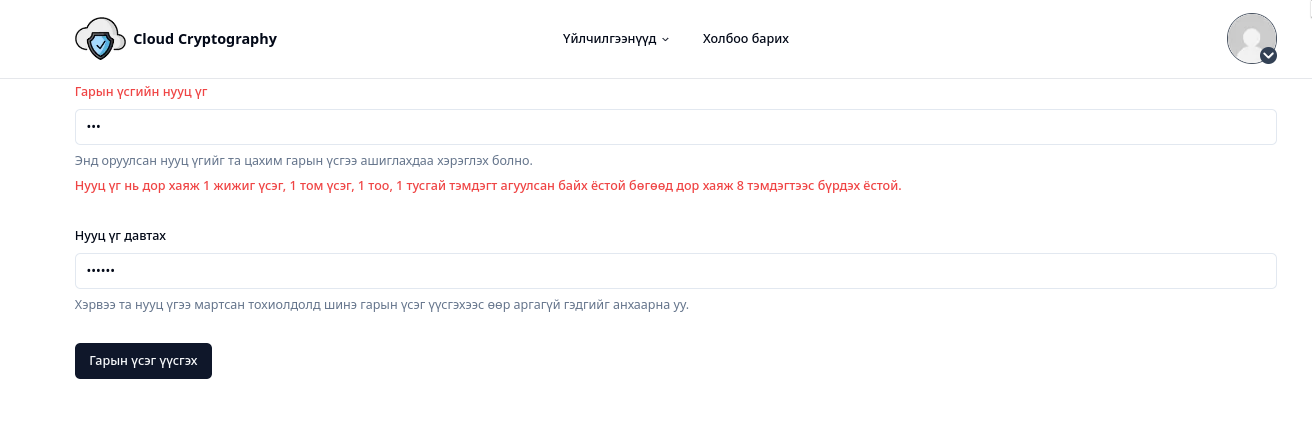
\includegraphics[scale=0.45]{assets/web/makepass.png}
	\caption{Тоон гарын үсэг үүсгэх шаардлага}
	\label{fig:architecture}
\end{figure}
\begin{figure}[h]
	\centering
	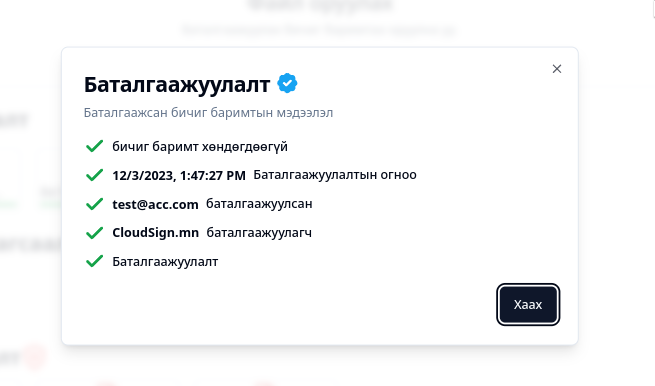
\includegraphics[scale=0.55]{assets/web/batalgaajuulaltConfirmed.png}
	\caption{Хүчинтэй гарын үсэгтэй баримт}
	\label{fig:architecture}
\end{figure}
\begin{figure}[h]
	\centering
	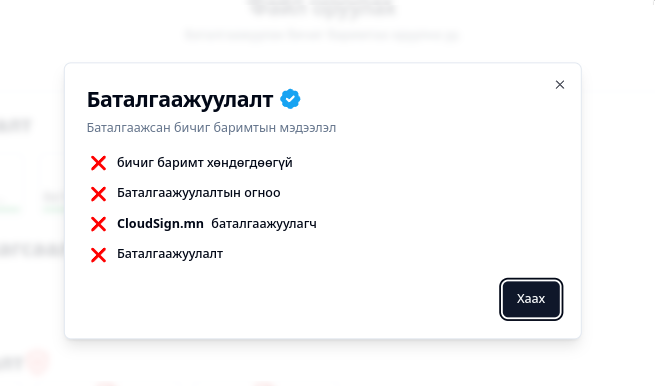
\includegraphics[scale=0.55]{assets/web/batalgaajuulaltDeclined.png}
	\caption{Хүчингүй гарын үсэгтэй баримт}
	\label{fig:architecture}
\end{figure}
\begin{figure}[h]
	\centering
	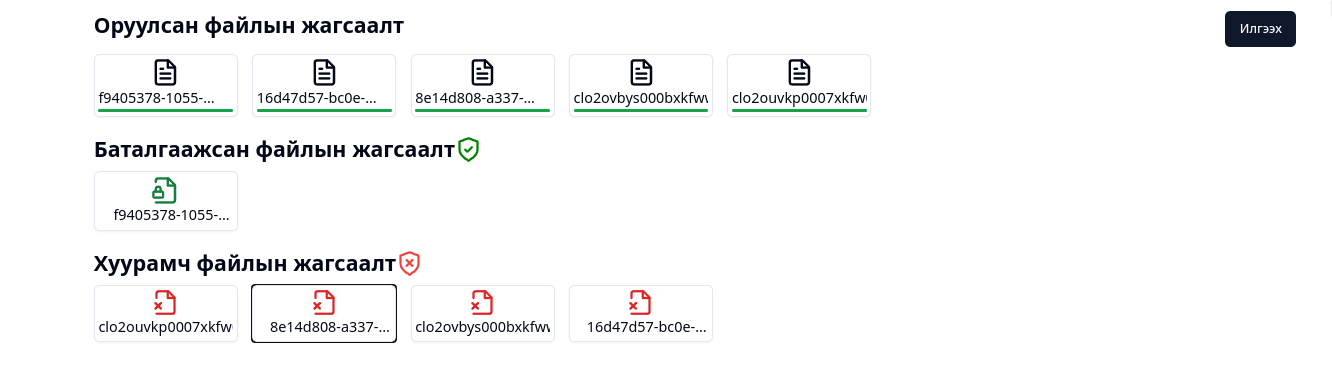
\includegraphics[scale=0.5]{assets/web/list.png}
	\caption{Нийт баримтын жагсаалт}
	\label{fig:architecture}
\end{figure}
\begin{figure}[h]
	\centering
	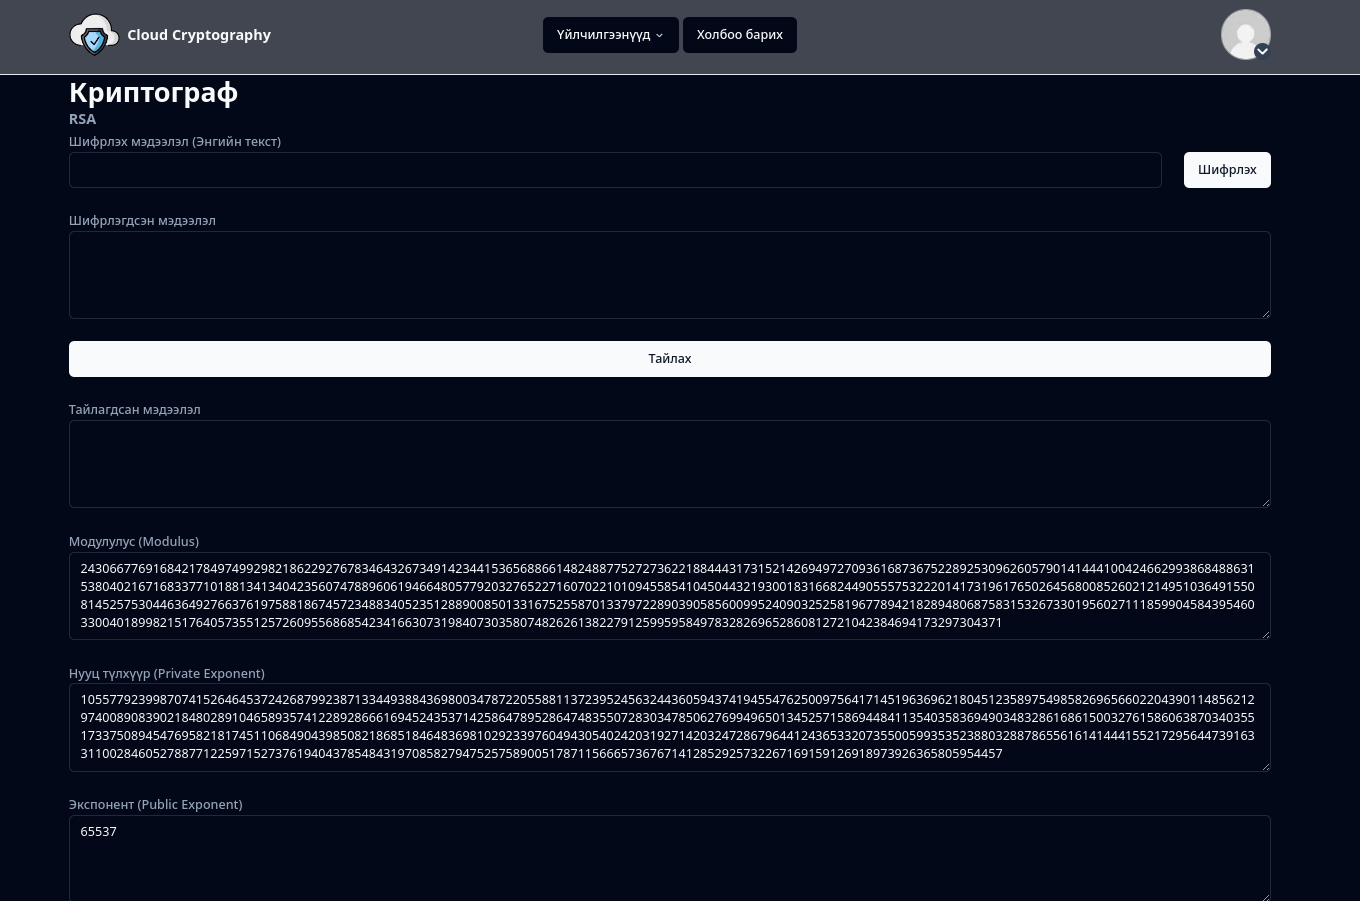
\includegraphics[scale=0.35]{assets/web/rsa.png}
	\caption{РСА (RSA) алгоритмын хэрэгжүүлэлт}
	\label{fig:architecture}
\end{figure}

\begin{figure}[h]
	\centering
	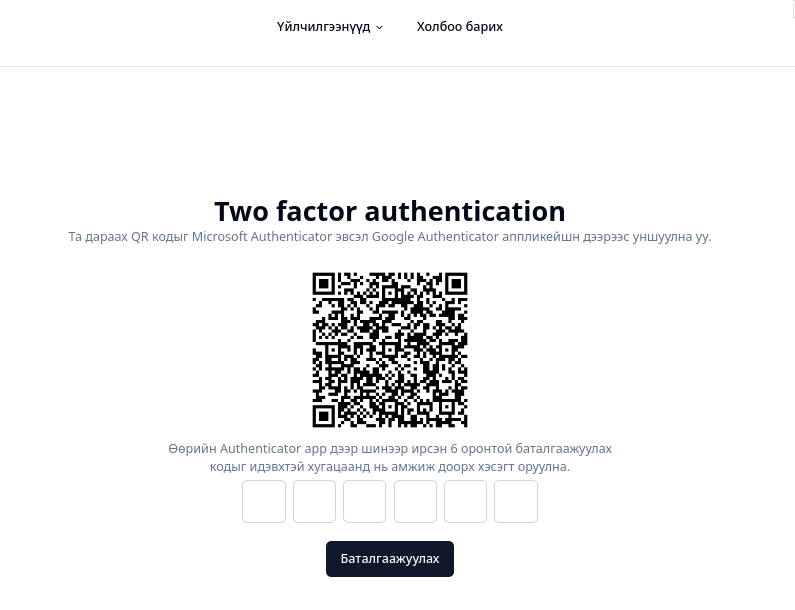
\includegraphics[scale=0.55]{assets/web/2fa.png}
	\caption{Цагаас хамаарсан нууц үг тохируулах}
	\label{fig:architecture}
\end{figure}
\begin{figure}[h]
	\centering
	
\includegraphics[scale=0.65]{assets/web/2faconfirm.png}
	\caption{Цагаас хамаарсан нууц үг тохируулсны дараа}
	\label{fig:architecture}
\end{figure}



% \chapter{Тайлан боловсруулах зөвлөмж}
% \subfile{writing.tex}


%----------------------------------------------------------------------------------------
%   Дүгнэлт эндээс эхэлнэ
%----------------------------------------------------------------------------------------
\conclusion{Дүгнэлт}
Дүгнэлт дууссаны дараа бичигдэнэ.


%----------------------------------------------------------------------------------------
%   Дипломын номзүй, хавсралтын хэсэг эндээс эхэлнэ
%----------------------------------------------------------------------------------------

\singlespace
\addcontentsline{toc}{part}{НОМ ЗҮЙ}
\begin{thebibliography}{}
	% Ашигласан материалыг эндээс оруулна
	\bibitem{AES}
	Daemen, J., \& Rijmen, V. (2002). "The Design of Rijndael: AES - The Advanced Encryption Standard." Springer. p.1-2.
	\bibitem{pharagraph1}
	Paragraphs and new lines,  Share LaTex, \url{https://www.sharelatex.com/learn/Paragraphs_and_new_lines}
	\bibitem{intro_crypo}
	Д. Гармаа (2022). "Криптографын үндэс." Улаанбаатар хот.
	\bibitem{modern_crypto}
	Bellare, Mihir; Rogaway, Phillip (11 May 2005), Introduction to Modern Cryptography (Lecture notes), archived (PDF) from the original on 2023-10-30, chapter 3.
	\bibitem{Reactjs}
	ReactJS, \url{https://reactjs.org/}
	

\end{thebibliography}


%----------------------------------------------------------------------------------------
%   Хавсралтууд эндээс эхэлнэ
%----------------------------------------------------------------------------------------
\appendix
\addcontentsline{toc}{part}{ХАВСРАЛТ}

% Хавсралтын нэр. Хавсралт гэдэг үг агуулахгүй
% \chapter{Шинжилгээ зохиомж}
% Хавсралтын агуулга

% Хавсралтын нэр. Хавсралт гэдэг үг агуулахгүй
% \chapter{Кодын хэрэгжүүлэлт}

% \lstinputlisting[language=Typescript, caption=tRPC тохиргоо,label=lst:trpc,frame=single]{src/code/trpc.ts}

% \lstinputlisting[language=yaml, caption=Docker Compose ,label=lst:docker-compose,frame=single]{src/code/docker-compose.yml}



\end{document}
